\chapter{Aspectos Teóricos}

% TODO: escribir la idea general

\noindent
En este capítulo cimentamos las bases teóricas necesarias para resolver instancias particulares de
programas lineales enteros. En primer lugar, la sección de prerrequisitos recopila resultados
básicos de teoría de números y de programación lineal que constituyen las herramientas principales para la
derivación de nuestros propios resultados. En segundo lugar, la sección de Fundamentos comienza con
definiciones y enunciados obtenidos de \cite{herr}, los cuales utilizaremos para continuar con la
construcción de nuestros resultados que, en pleno conocimiento del autor, son originales. El
problema fundamental que permitirá construir incrementalmente nuestro algoritmo es
\begin{subequations}
	\label{theory:formulation}
	\begin{align}
		\max_{\vec{x} \in \Z^n} \quad
			& \vec{p}^T\vec{x}, \label{theory:objective} \\
		\text{s.a.} \quad
			& \vec{p}^T\vec{x} \leq u, \label{theory:constraint:budget} \\
			& \vec{x} \geq \vec{0}. \nonumber
	\end{align}
\end{subequations}

En la sección de Fundamentos analizaremos a profundidad este problema, cuyo punto de
culminación será el teorema \ref{theory:th:feasibility}. Veremos que es recomendable separar en dos
partes el análisis de este problema: el caso $p_i < 0$ para alguna $i \in \braces{1, \ldots, n}$; y
el caso $\vec{p} > \vec{0}$. Observemos que, para este problema, podemos suponer sin pérdida de
generalidad que todas las entradas de $\vec{p}$ son no nulas. Cuando introduzcamos múltiples
restricciones en la sección \ref{sec:multiple} nos desharemos de este supuesto.

Los siguientes dos capítulos examinarán respectivamente los casos que induce el teorema
\ref{theory:th:feasibility}. Por el momento, cabe destacar que el segundo caso será de mayor interés
y tendrá mayor aplicabilidad en problemas reales, pues es una instancia particular del Problema de
la Mochila. No obstante, el caso $p_i < 0$ para alguna $i \in \braces{1, \ldots, n}$ también será de
utilidad para exhibir casos particulares en donde el algoritmo de Ramificación y Acotamiento obtiene
un rendimiento deficiente.

\section{Prerrequisitos}
\label{sec:prerreq}
\noindent
En los siguientes capítulos usaremos extensivamente resultados básicos de teoría de números y de
programación lineal, por lo que es provechoso recopilarlos en esta primera sección. En
particular, destaca la importancia de las ecuaciones lineales diofantinas para la construcción
de nuestro algoritmo. En esta sección el autor consideró pertinente no incluir demostraciones, pues los
enunciados son mostrados en cualquier clase de álgebra superior, programación lineal, o
investigación de operaciones, por ejemplo. La referencia principal para la parte de teoría de
números es \cite{carmen}, mientras que la de programación lineal es \cite{fabs}.

\subsection{Teoría de Números}
\label{section:number-theory}
\subsubsection{Máximo común divisor y mínimo común múltiplo}
\noindent
En primer lugar, introducimos el símbolo de relación ``$\mid$'' para indicar divisibilidad. Dados
dos enteros $a, b$, decimos que $b$ divide a $a$ (y escribimos $b \mid a$) si y solo si existe un
entero $k$ tal que $a = k \cdot b$. Así también, denotamos el conjunto de divisores de $a$ como
\begin{equation*}
	D(a) \coloneq \lbrace b \in \Z \vcentcolon b \mid a \rbrace.
\end{equation*}
Si $a$ es distinto de cero, encontramos que $D(a)$ es finito, puesto que si $b \mid a$, entonces
$|b| \leq |a|$, lo cual implica que $|D(a)| \leq 2|a|$. En caso de que $a$ sea nulo, obtenemos $D(a)
= \Z$. Observemos también que $\lbrace -1, 1 \rbrace \subseteq D(a)$ para todo entero $a$.

\begin{definition}
	\label{prerreq:def:gcd}
	Sean $a_1, \ldots, a_n$ enteros no todos iguales a cero, entonces definimos su \textbf{máximo
	común divisor} $d$ como el elemento maximal del conjunto $\bigcap_{i=1}^{n}D(a_i)$, y escribimos
	$d = \gcd{a_1, \ldots, a_n}$. Si $d = 1$, entonces decimos que $a_1, \ldots, a_n$ son
	\textbf{coprimos}.
\end{definition}

Puesto que $a_i \neq 0$ para alguna $i$ en la definición anterior, encontramos que el conjunto
$\bigcap_{i=1}^{n}D(a_i)$ es finito y, como también es no vacío, en efecto existe un elemento maximal.
Es decir, el máximo común divisor $d$ siempre está bien definido. Cabe mencionar que el máximo común
divisor siempre es estrictamente positivo, pues se cumple que $1 \in D(a)$ para todo entero $a$.

Otra definición equivalente para el máximo común divisor normalmente es dada de manera inductiva.
Decimos que $d$ es el máximo común divisor de dos enteros $a_1, a_2$, no ambos nulos, si se
satisface
\begin{enumerate}
	\item $d \mid a_1$ y $d \mid a_2$, y también,
	\item si $d' \mid a_1$ y $d' \mid a_2$, entonces $d' \mid d$.
\end{enumerate}
Luego, para un conjunto de enteros $a_1, a_2 \ldots a_n$, no todos nulos, definimos el máximo común
divisor entre ellos a partir de
\begin{equation*}
	\gcd{a_1, a_2, \ldots, a_{n-1}, a_n} \coloneq \gcd{a_1, \gcd{a_2, \ldots, \gcd{a_{n-1}, a_n}}}.
\end{equation*}
Sin embargo, debemos ser cuidadosos con esta manera de definir las cosas, pues puede ser el caso,
por ejemplo, que $a_{n-1} = a_n = 0$ y entonces $\gcd{a_{n-1}, a_n}$ no está bien definido. Una
manera simple de arreglar esto último es agregar la condición de que $a_n$ sea no nulo. Es por esto
último que el autor prefirió la definición \ref{prerreq:def:gcd}. Independientemente de cómo
definamos el máximo común divisor, la manera de calcularlo siempre es a través del Algoritmo de
Euclides. A partir de este punto usaremos ambas definiciones de manera indistinta.

\begin{observation}
	No porque una colección de enteros sea coprima se sigue que estos enteros son coprimos a pares.
	Por ejemplo, los enteros 1, 3 y 3 son coprimos pero evidentemente 3 y 3 no lo son.
\end{observation}

\begin{definition}
	Decimos que $c \in \Z$ es una \textbf{combinación lineal entera} de un conjunto de enteros $a_1, \ldots,
	a_n$ si existen enteros $x_1, \ldots, x_n$ tales que $c = a_1x_1 + \cdots + a_nx_n$. Si $c$ es
	positivo, también decimos que esto último es una \textbf{combinación lineal entera positiva}.
\end{definition}

El siguiente teorema, a pesar de su simpleza, es central para los resultados obtenidos en esta
tesis.
\begin{theorem}
	\label{prerreq:th:bezout}
	Sea $d$ un entero y sean $a_1, \ldots, a_n$ una colección de enteros no todos iguales a cero.
	Entonces $d = \gcd{a_1, \ldots, a_n}$ si y solo si $d$ es la mínima combinación lineal entera
	positiva de $a_1, \ldots, a_n$.
\end{theorem}

\begin{example}
	El maximo común divisor $d$ de los enteros $a_1 \coloneq 2$, $a_2 \coloneq 3$ y $a_3 \coloneq 5$
	es 1 y además se cumple que $-3a_1 - a_2 + 2a_3 = 1 = d$.
\end{example}

\begin{lemma}
	\label{prerreq:lemma:gcd}
	Si $d = \gcd{a_1, \ldots, a_n}$, entonces $\gcd{\frac{a_1}{d}, \ldots, \frac{a_n}{d}} = 1$.
\end{lemma}

Además del máximo común divisor, requeriremos al mínimo común múltiplo, empero en menor medida. Sea
$a$ un entero y denotamos el conjunto de sus múltiplos como
\begin{equation*}
	M(a) \coloneq \lbrace x \in \Z \vcentcolon a \mid x \rbrace.
\end{equation*}
Si $a$ es nulo, entonces $M(a) = \lbrace 0 \rbrace$. En caso contrario encontramos que $M(a)$ es un
conjunto infinito. Ánalogamente a la definición \ref{prerreq:def:gcd}, definimos el mínimo común
múltiplo $m$ de una colección de enteros $a_1, \ldots, a_n \in \Z \setminus \lbrace 0 \rbrace$ como
el elemento minimal de $\N \cap \bigcap_{i=1}^{n}M(a_i)$. Escribimos $m = \lcm{a_1, \ldots, a_n}$.
Para observar que está bien definido, basta mencionar que el producto $|a_1 \cdots a_n|$ es un
elemento de la intersección y por lo tanto esta es no vacía.

\subsubsection{Ecuaciones lineales diofantinas}

\noindent
Sea $c \in \Z$ y sean $a_1, \ldots, a_n$ enteros. Una ecuación lineal diofantina es una ecuación
donde queremos encontrar enteros $x_1, \ldots, x_n$ que satisfagan
\begin{equation*}
	a_1x_1 + \cdots + a_nx_n = c.
\end{equation*}
Será de nuestro interés en las siguientes secciones resolver iterativamente este tipo de ecuaciones.
Por el momento basta mencionar que podemos enfocarnos en el caso $n = 2$ sin ninguna pérdida de
generalidad. No obstante, los resultados se mantienen para cualquier $n \in \N$. Los siguientes
enunciados abordan el problema de determinar existencia y unicidad para las ecuaciones lineales
diofantinas, así como la construcción de sus soluciones.

\begin{theorem}[Existencia]
	\label{prerreq:th:existence}
	Sean $a, b \in \Z$, no ambos cero. La ecuación $ax + by = c$ tiene solución entera si y solo si
	$\gcd{a, b} \mid c$.
\end{theorem}

Para construir el conjunto de soluciones a una ecuación lineal diofantina, encontramos primero una
solución particular.
\begin{definition}
	\label{prerreq:def:bezout}
	Sea $d \coloneq \gcd{a, b}$ y sean $x', y'$ enteros tales que $ax' + by' = d$ (c.f. teorema
	\ref{prerreq:th:bezout}). Decimos entonces que $x', y'$ son \textbf{coeficientes de Bézout} asociados a
	$a, b$, respectivamente\footnote{
		Los coeficientes de Bézout se pueden calcular a través del Algoritmo Extendido de Euclides.
		Véase \url{https://en.wikipedia.org/wiki/Extended_Euclidean_algorithm}.
	}.
\end{definition}

\begin{observation}
	Los coeficientes de Bézout asociados a un par de enteros no son únicos. En efecto, si $x', y'$
	son coeficientes de Bézout de $a, b$, entonces $x' + b$, $y' - a$ también lo son:
	\begin{equation*}
		a(x' + b) + b(y' - a) = ax' + by' + ab - ab = ax' + by' = d.
	\end{equation*}
	Para fines de esta tesis basta la existencia de estos coeficientes, por lo que decimos de manera
	indistinta ``los coeficientes de Bézout'' y ``una elección de coeficientes de Bézout''.
\end{observation}

Definamos $d \coloneq \gcd{a, b}$ y supongamos que la ecuación $ax + by = c$ tiene solución.
Por el teorema \ref{prerreq:th:existence}, se sigue que $d \mid c$, y entonces existe $c' \in \Z$
tal que $c = c' \cdot d$. Sean $x', y'$ los coeficientes de Bézout asociados a $a, b$
respectivamente. Así,
\begin{equation*}
	a(c' \cdot x') + b(c' \cdot y') = c'(ax' + by') = c'd = c,
\end{equation*}
por lo que $(c' \cdot x', c' \cdot y')$ es una solución particular de la ecuación $ax + by = c$.

\begin{theorem}[Construcción]
	\label{prerreq:th:construction}
	Sea $(x_0, y_0)$ una solución particular de la ecuación lineal diofantina $ax + by = c$.
	Entonces todas las soluciones de la ecuación están dadas por
	\begin{equation}
		\label{prerreq:eq:construction}
		\begin{cases}
			x = x_0 + \frac{b}{d}t, \\
			y = y_0 - \frac{a}{d}t,
		\end{cases}
	\end{equation}
	donde $d \coloneq \gcd{a, b}$ y $t \in \Z$.
\end{theorem}

\begin{example}
	Consideremos la ecuación lineal $2x + 3y = 5$. Los coeficientes de Bézout asociados a 2 y 3 son,
	respectivamente, -1 y 1. Luego, una solución particular para la ecuación es $(x_0, y_0) = (-5, 5)$.
	Por el teorema anterior encontramos que todas las soluciones están dadas por
	\begin{equation*}
		\begin{cases}
			x = -5 + 3t, \\
			y = 5 - 2t,
		\end{cases}
	\end{equation*}
	donde $t \in \Z$ es una variable libre. En efecto, sustituyendo obtenemos
	\begin{equation*}
		2(-5 + 3t) + 3(5 - 2t) = -10 + 15 + 6t - 6t = 5.
	\end{equation*}
\end{example}

\subsection{Programación lineal}
\noindent
La programación lineal se encarga de resolver problemas de optimización de la forma
\begin{equation}
	\label{prim:lineal-opt}
	\max_{\vec{x}} ~\lbrace \vec{c}^T\vec{x} \colon \vec{x} \in P \rbrace,
\end{equation}
donde $P$ es un poliedro. En esta sección repasamos brevemente propiedades del poliedro $P$ al cual
llamamos región factible. Así también, indicamos dónde se encuentra el óptimo del problema y
hacemos mención rápida sobre cómo obtenerlo. Finalmente, nos enfocamos en programas lineales enteros
y, más importantemente, describimos cómo funciona el algoritmo de Ramificación y Acotamiento para
encontrar sus soluciones.

\begin{definition}
	Sea $\vec{a} \in \R^n$ un vector no nulo y sea $b \in \R$ un escalar. Llamamos
	\textbf{hiperplano afino}
	al conjunto de vectores $\vec{x} \in \R^n$ que satisfacen $\vec{a}^T\vec{x} = b$. Así también,
	llamamos \textbf{semi-espacios afinos} a los conjuntos de vectores $\vec{x}, \vec{y} \in \R^n$ que
	satisfacen $\vec{a}^T\vec{x} \geq b$ y $\vec{a}^T\vec{y} \leq b$.
\end{definition}

\begin{definition}
	Sea $A \in \R^{m \times n}$ una matriz con renglones linealmente independientes y $\vec{b} \in
	\R^m$ un vector. Entonces al conjunto definido por
	\begin{equation}
		\label{prerreq:def:poly}
		P \coloneq \lbrace \vec{x} \in \R^n \colon A\vec{x} \geq \vec{b} \rbrace
	\end{equation}
	lo llamamos \textbf{poliedro}. Si, además, $P$ es acotado, entonces decimos que $P$ es un
	\textbf{politopo}.
\end{definition}

\begin{observation}
	Todo poliedro $P$ definido de esta manera representa la intersección de $m$ semi-espacios
	afinos. Esto se debe a que $A\vec{x} \geq \vec{b}$ si y solo si $\vec{a}_i^T\vec{x} \geq b_i$
	para toda $1 \leq i \leq m$ y donde $\vec{a}_i^T$ representa el $i$-ésimo renglón de la matriz
	$A$. En la Figura \ref{fig:hyp} se muestra visualmente esta relación entre hiperplanos afinos y
	poliedros.
\end{observation}

\begin{figure}[ht]
	\centering
	\begin{minipage}{0.45\textwidth}
		\centering
		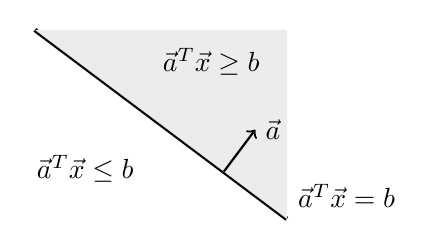
\begin{tikzpicture}[scale=0.8]
			% hyperplane
			\draw[ultra thick, black] (-2,1) -- (2,-2) node[above right] {$\vec{a}^T\vec{x} = b$};
			% labels
			\node at (-1.2,-1.2) {${\vec{a}^T \vec{x} \leq b}$};
			%shading
			\fill[gray!15, domain=-2:2, variable=\x]
				(-2,1) -- plot ({\x}, {-0.75*\x - 0.5}) -- (2,1) -- cycle;
			\draw[->, thick] (1,-1.25) -- (1.5,-0.583) node[right] {$\vec{a}$};
			\node at (0.8,0.5) {${\vec{a}^T \vec{x} \geq b}$};
		\end{tikzpicture}
	\end{minipage}
	\begin{minipage}{0.45\textwidth}
		\centering
		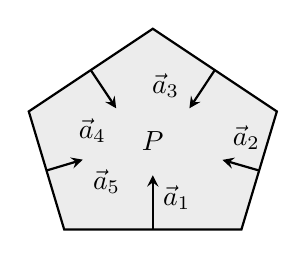
\begin{tikzpicture}[scale=1.5, >=stealth]
			% coordinates
			\coordinate (A) at (0,0);
			\coordinate (B) at (1.5,0);
			\coordinate (C) at (1.8,1);
			\coordinate (D) at (0.75,1.7);
			\coordinate (E) at (-0.3,1);
			% pentagon
			\filldraw[fill=gray!15, thick]
			(A) -- (B) -- (C) -- (D) -- (E) -- cycle;
		  % normal vectors
			% AB
			\draw[->, black, thick] (0.75,0) -- (0.75,0.46) node[below right] {$\vec{a}_1$};
			% BC
			\draw[->, black, thick] (1.65,0.5) -- (1.34,0.59) node[above right] {$\vec{a}_2$};
			% CD
			\draw[->, black, thick] (1.275,1.35) -- (1.06,1.027) node[above left] {$\vec{a}_3$};
			% DE
			\draw[->, black, thick] (0.225,1.35) -- (0.44,1.027) node[below left] {$\vec{a}_4$};
			% EA
			\draw[->, black, thick] (-0.15,0.5) -- (0.157,0.592) node[below right] {$\vec{a}_5$};
			% polyhedron label
			\node at (0.75, 0.75) {$P$};
		\end{tikzpicture}
	\end{minipage}
	\caption{\textit{Izquierda:} Un hiperplano afino $\braces{\vec{x} \colon \vec{a}^T\vec{x} = b}$
	junto con los dos semi-espacios que induce. \textit{Derecha:} Este poliedro $P$ es acotado y es
	la intersección de un conjunto finito de semi-espacios inducidos por un hiperplano afino.}
	\label{fig:hyp}
\end{figure}

\begin{definition}
	Sea $P$ un poliedro. Decimos que el vector $\vec{x} \in P$ es un \textbf{vértice} de $P$ si existe
	$\vec{c} \in \R^n$ de manera que $\vec{c}^T\vec{x} < \vec{c}^T\vec{y}$ para todo $\vec{y} \in P
	\setminus \lbrace \vec{x} \rbrace$.
\end{definition}
En términos gráficos, decimos que $\vec{x}$ es un vértice si se satisfacen dos condiciones: en
primer lugar, existe un hiperplano afino que pasa por $\vec{x}$ y uno de sus semi-espacios inducidos
contiene completamente al poliedro $P$; en segundo lugar, ningún otro punto de $P$ se encuentra
sobre este hiperplano.

\begin{definition}
Sea $P$ un poliedro y sea $\vec{c} \in \R^n$ un vector. Todo problema de optimización de la forma
\eqref{prim:lineal-opt} entra en una de las siguientes tres categorías:
\begin{enumerate}
	\item El valor óptimo no existe: ningún vector $\vec{x} \in \R^n$ satisface
		el sistema de desigualdades $A\vec{x} \geq \vec{b}$. Es decir, la región factible es vacía.
	\item El valor óptimo existe y es infinito: el poliedro $P$ no es acotado y
		somos capaces de encontrar una sucesión de vectores $\lbrace \vec{x}_k \rbrace_{k \in \N}$
		en el poliedro $P$ que satisface $\vec{c}^T\vec{x}_{k+1} > \vec{c}^T\vec{x}_k$ para todo $k \in \N$.
	\item El valor óptimo existe y es finito: este caso es la negación de los dos casos anteriores,
		pero cabe recalcar que esto no significa que el poliedro $P$ es acotado.
\end{enumerate}
En el primer caso decimos que \textbf{el problema es infactible}, mientras que en los últimos dos
decimos que \textbf{el problema es factible}. También diremos comúnmente del segundo caso que
\textbf{el problema es no acotado}.
\end{definition}

Es posible mostrar que todo poliedro $P \coloneq \lbrace \vec{x} \in \R^n \colon A\vec{x} \geq
\vec{b} \rbrace$ puede ser transformado a la forma estándar
\begin{equation*}
	\lbrace \left( \vec{x}^+, \vec{x}^-, \vec{s} \right) \in \R^{n + n + m} \colon A(\vec{x}^+ -
\vec{x}^-) - \vec{s} = \vec{b}, \left(\vec{x}^+, \vec{x}^-, \vec{s}\right) \geq \vec{0}\rbrace,
\end{equation*}
de manera que todo problema de optimización de la forma \eqref{prim:lineal-opt} puede ser escrito
sin pérdida de generalidad como
\begin{subequations}
	\label{prerreq:formulation}
	\begin{align}
		\max_{\vec{x} \in \R^n} \quad
			& \vec{c}^T\vec{x}, \label{prerreq:formulation:objective} \\
		\text{s.a.} \quad
			& A\vec{x} = \vec{b}, \label{prerreq:formulation:constraints} \\
			& \vec{x} \geq \vec{0} \nonumber,
	\end{align}
\end{subequations}
donde ``s.a.'' es una abreviación de ``sujeto a''. De ahora en adelante, nuestro análisis se
concentrará exclusivamente en problemas lineales de este tipo. Es decir, supondremos, sin pérdida de
generalidad, que todo problema lineal se encuentra en esta forma estándar.

\begin{theorem}
	\label{prerreq:th:linear-sol}
	Sea $P$ un poliedro que tiene al menos un vértice, consideremos el problema
	\eqref{prerreq:formulation}, y supongamos que el valor óptimo $z^*$ existe y es finito. Entonces
	el conjunto de soluciones óptimas contiene al menos un vértice de $P$.
\end{theorem}

Este teorema fundamental constituye el primer paso para la construcción de varios algoritmos que
encuentran soluciones del problema \eqref{prerreq:formulation}. Ciertamente el más famoso de todos
es el algoritmo simplex, el cual ``salta'' de vértice en vértice hasta llegar a uno con valor
óptimo. Otros, más modernos y conocidos como métodos de puntos interiores, comienzan en el interior
del poliedro $P$ y son ``atraídos'' como imanes a uno de los vértices con valor óptimo. No es el
objetivo de esta tesis exponer la maquinaria matemática detrás de estos algoritmos\footnote{
	Sin embargo, la literatura para explicar estos métodos es harto abundante. Véase, por ejemplo,
	\cite{nocedal}.
}.

Ahora describimos brevemente los programas lineales enteros y pasamos a explicar el método de
Ramificación y Acotamiento. Por ello, lo que se encuentra a continuación supone que contamos con un
algoritmo para resolver problemas del tipo \eqref{prerreq:formulation}.
\begin{definition}
	Sea $A \in \R^{m \times n}$ una matriz con renglones linealmente independientes y sea $\vec{b}
	\in \R^m$ un vector. Al problema de optimización lineal \eqref{prerreq:formulation} lo llamamos
	\textbf{problema relajado} del programa lineal entero
	\begin{subequations}
		\label{prerreq:formulation:ilp}
		\begin{align}
			\max_{\vec{x} \in \Z^n} \quad
				& \vec{c}^T\vec{x}, \label{prerreq:formulation:objective:ilp} \\
			\text{s.a.} \quad
				& A\vec{x} = \vec{b}, \label{prerreq:formulation:constraints:ilp} \\
				& \vec{x} \geq \vec{0} \nonumber.
		\end{align}
	\end{subequations}
\end{definition}
Resalta el hecho de que la formulación de un programa lineal entero es idéntico a su formulación
relajada, solamente agregamos la restricción de que nuestro vector solución $\vec{x}^*$
sea entero. Es decir, lo único que cambia es la región de factibilidad. De hecho, si
definimos el poliedro
\begin{equation*}
	P \coloneq \lbrace \vec{x} \in \R^n \colon A\vec{x} = \vec{b}, \vec{x} \geq \vec{0} \rbrace,
\end{equation*}
entonces tenemos que $P \cap \Z^n$ corresponde a la región factible de
\eqref{prerreq:formulation:ilp}, mientras que $P$ corresponde a la región factible de su problema
relajado.

A partir de lo anterior, deducimos inmediatamente que el valor óptimo $\optilp{z}$ de un programa
entero es una cota inferior del valor óptimo $z^*$ de su problema relajado, pues ambos son problemas
de maximización y es cierto que $P \cap \Z^n \subseteq P$. De aquí se sigue entonces que si $z^* =
\optilp{z}$, entonces la solución óptima $\vec{x}^*$ del problema relajado también es la solución
óptima del programa lineal entero.

Para resolver problemas lineales enteros más generales, comúnmente se utiliza el algoritmo de
Ramificación y Acotamiento. Este método consiste en generar un árbol binario donde cada nodo
representa un subproblema lineal a resolver. En la raíz del árbol resolvemos el problema relajado
\eqref{prerreq:formulation} y, si la solución óptima $\vec{x}^* \in \R^n$ no es entera, entonces
para alguna entrada $x_i^*$ no entera agregamos la restricción $x_i \leq \lfloor x_i^* \rfloor$ para
crear un subproblema, y también añadimos la restricción $x_i \geq \lceil x_i^* \rceil$ para crear
otro subproblema. Este procedimiento se realiza de manera recursiva.

Observemos que, si decidimos recorrer todos los nodos del árbol binario, entonces tendremos que
resolver al menos $2^n$ subproblemas, donde $n$ es la dimensión del problema lineal. Por esta razón,
el algoritmo cuenta con políticas para deshacerse de subárboles que nunca proveerán la solución
óptima. El autor considera que es mejor ilustrar estas políticas a partir de un ejemplo. El
Algoritmo \ref{algo:bb} en el Apéndice \ref{app:bb} presenta una versión rudimentaria del método de
Ramificación y Acotamiento.

\begin{example}[\cite{fabs}]
	\label{ex:ilp}
	Consideremos el programa lineal entero
	\begin{align*}
		\max_{\vec{x} \in \Z^2} \quad
			& 4x_1 - x_2, \\
			\text{s.a.} \quad
			& 7x_1 - 2x_2 \leq 14, \\
			& 2x_1 - 2x_2 \leq 3, \\
			& x_2 \leq 3, \\
			& x_1, x_2 \geq 0.
	\end{align*}
	La región factible de este problema se muestra en la Figura \ref{fig:feas}. La solución al problema
	relajado, cuya región factible denotamos por $S_0$, está dada por $\vec{x}^0 \coloneq (20/7,
	3)^T$. Como $x_1^0 = 20/7$ no es entero, generamos dos nuevos subproblemas con regiones
	factibles
	\begin{align*}
		S_{00} &\coloneq S_0 \cup \braces{ x_1 \leq \floor{20/7} = 2}, \\
		S_{01} &\coloneq S_0 \cup \braces{ x_1 \geq \ceil{20/7} = 3}.
	\end{align*}
	De la Figura \ref{fig:feas}, observamos que $S_{01}$ es vacío y por lo tanto de este problema no
	podemos generar otros subproblemas. En este caso, decimos que \textbf{podamos $S_{01}$ por
	infactibilidad}.

	Ahora bien, la solución al problema $S_{00}$ está dada por $\vec{x}^1 \coloneq (2, 1/2)^T$.
	Encontramos que $x_2^1$ = 1/2 no es entero y por lo tanto generamos dos nuevos subproblemas:
	\begin{align*}
		S_{000} &\coloneq S_{00} \cup \braces{ x_2 \leq \floor{1/2} = 0}, \\
		S_{001} &\coloneq S_{00} \cup \braces{ x_2 \geq \ceil{1/2} = 1}.
	\end{align*}
	Observemos que la solución $\vec{x}^2$ de $S_{001}$ es $(2, 1)^T$, la cual es entera y tiene valor
	objetivo $z_2^* \coloneq 7$. No generamos otros subproblemas a partir de este problema porque
	sus regiones factibles estarán contenidas en $S_{001}$ y por lo tanto sus valores objetivos
	serán menores o iguales al de $S_{001}$. Así pues, decimos que \textbf{podamos $S_{001}$ por
	integralidad}.

	La solución de $S_{000}$, en cambio, es $\vec{x}^3 \coloneq (3/2, 0)^T$ y tendríamos que ramificar
	de nuevo en otros dos subproblemas. No obstante, observemos que el valor objetivo de este
	subproblema es $z_3^* \coloneq 6$, el cual es menor que $z_2^* = 7$. Como la región factible de
	cualquier subproblema generado a partir de este último problema estára contenido en $S_{000}$,
	se sigue que su valor objetivo será menor o igual al de $S_{000}$ Decimos entonces que
	\textbf{podamos $S_{000}$ por cota}.

	Como hemos agotado todos los subproblemas que podríamos generar, entonces concluimos que la
	solución óptima de este programa  lineal entero es $\vec{x}^2 = (2, 1)^T$ y tiene valor objetivo
	$z_2^* = 7$.
\end{example}
\begin{figure}
	\centering
	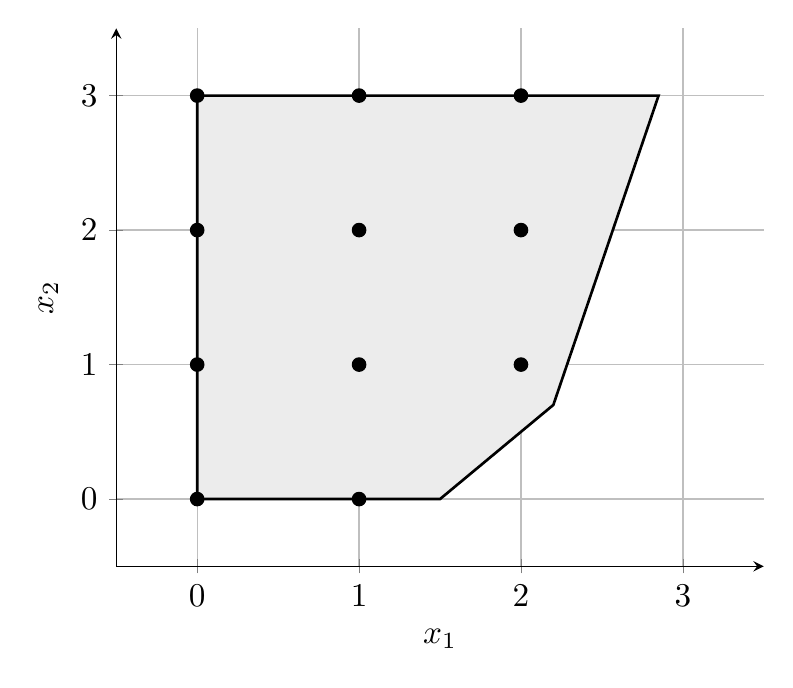
\begin{tikzpicture}[scale=1.2]
		\begin{axis}[
			axis lines=left,
			xmin=-0.5, xmax=3.5,
			ymin=-0.5, ymax=3.5,
			grid=both,
			xlabel=$x_1$,
			ylabel=$x_2$
			]
			\addplot+ [thick,color=black,fill=gray!15,mark=none] table {
				0 0
				1.5 0
				2.2 0.7
				2.85 3
				0 3
				0 3
				0 0
			};
			\addplot+ [only marks,,mark=*,mark options={scale=1, color=black, fill=black}] table {
				0 0
				0 1
				0 2
				0 3
				1 0
				1 1
				1 2
				1 3
				2 1
				2 2
				2 3
			};
		\end{axis}
	\end{tikzpicture}
	\caption{Los puntos negros forman la región factible del programa lineal entero del Ejemplo
	\ref{ex:ilp}, mientras que la región sombreada es la región factible de su problema relajado.}
	\label{fig:feas}
\end{figure}

\section{Fundamentos}
\noindent
Esta sección constituye el primer paso para la construcción de nuestro algoritmo. Se divide en dos
partes. Primeramente damos a conocer las definiciones y enunciados provistos por \cite{herr}, al
mismo tiempo que hacemos un par de observaciones. Esta primera parte puede darse por concluida una
vez citado el teorema \ref{phase-1:th:cover}. Así también, es importante aclarar que el autor
tradujo libremente algunos términos a falta de encontrar fuentes en español que hicieran uso de
ellos. A saber, el autor decidió nombrar ``vectores esencialmente enteros'' a los
\textit{projectively rational vectors} y ``capas enteras'' a los \textit{c-layers} en las
Definiciones \ref{theory:def:rational} y \ref{phase-1:def:c-layer}, respectivamente.

En la segunda parte de esta sección comenzamos con nuestro análisis del problema
(\ref{theory:formulation}). La razón de considerarlo fundamental para esta tesis fue mencionado en
el capítulo de Motivación, pero lo repetimos una vez más: en esta clase de problemas el vector es
ortogonal a la única restricción, y esto implica que el problema relajado tenga una infinidad de
soluciones. Hemos observado que, en presencia de este fenómeno, el algoritmo de Ramificación y
Acotamiento no divide la región factible de manera óptima. Por ello investigamos formas alternativas
para atacar este problema antes de hacer la separación de casos $p_i \leq 0$ para alguna $i \in
\lbrace 1, \ldots, n \rbrace$ o $\vec{p} > \vec{0}$.
\begin{definition}
	\label{theory:def:rational}
	Decimos que un vector $\vec{v} \in \R^n \setminus \lbrace \vec{0} \rbrace$ es \textbf{esencialmente
	entero} si existe un vector $\vec{w} \in \Z^n$ y un escalar $m \in \R \setminus \lbrace 0
	\rbrace$ tal que $\vec{v} = m\vec{w}$. Además, decimos que $\vec{w}$ es el \textbf{múltiplo
	coprimo} de $\vec{v}$ si sus entradas son coprimas (c.f. definición \ref{prerreq:def:gcd}) y si
	su primera entrada no nula $v_i$ también es positiva.
\end{definition}
En otras palabras, decimos que $\vec{v}$ es esencialmente entero si es un múltiplo real de un vector
entero.
\begin{example}
	El vector $\left(-\sqrt{2}, 1/\sqrt{2}\right)^T = \sqrt{2}(-1, 1/2)^T$ es esencialmente entero
	y $(2, -1)^T$ es su múltiplo coprimo. Contrariamente, el vector $(\sqrt{2}, \sqrt{3})^T$ no es
	esencialmente entero.
\end{example}
\begin{observation}
	Todo vector $\vec{v}$ cuyas entradas son racionales ($\vec{v} \in \Q^n$) es esencialmente
	entero. En efecto, $v_i = \frac{p_i}{q_i}$ para algunos enteros $p_i$ y $q_i$ con $q_i$
	distinto de cero. Si definimos $m \coloneq \lcm{q_1, \ldots, q_n} \neq 0$ y $\vec{w} \coloneq
	m\vec{v}$, se sigue que $\vec{v} = \frac{1}{m}\vec{w}$ y también $\vec{w} \in \Z^n$.
\end{observation}
\begin{observation}
	\label{obs:coprime-unique}
	Todo vector $\vec{v}$ esencialmente entero tiene a lo más dos vectores coprimos asociados. Sean
	$m \in \R$ y $\vec{w} \in \Z^n$ tales que $\vec{v} = m\vec{w}$. Entonces
	\begin{equation*}
		\pm \frac{1}{\gcd{w_1, \ldots, w_n}}\vec{w}
	\end{equation*}
	son dos vectores cuyas entradas son coprimas, de acuerdo al lema \ref{prerreq:lemma:gcd}. Como
	la primera entrada no nula $w_i$ también debe ser positiva, se sigue que solo uno de estos dos
	vectores es el múltiplo coprimo de $\vec{v}$. Así, el múltiplo coprimo de un vector
	esencialmente entero es único.
\end{observation}

Porque todo número representable en cualquier sistema de aritmética finita es necesariamente
racional, decidimos enfocar nuestro análisis en vectores esencialmente enteros. Desde el punto de
vista puramente teórico, esta condición reduce drásticamente el tipo de programas lineales que
podemos resolver. No obstante, esta clase de vectores es un poco más general que los considerados en
otros textos de programación lineal, por ejemplo, \cite{martello} y \cite{alex} toman en cuenta
vectores puramente racionales. En \cite{herr} se revelan propiedades de los vectores esencialmente
enteros que reproducimos aquí y que nos permitirán plantear ecuaciones lineales diofantinas cuyas
soluciones otorgan candidatos para puntos óptimos de un problema lineal.

\begin{definition}
	\label{phase-1:def:c-layer}
	Sea $\vec{v} \in \R^n$ un vector esencialmente entero y sea $t \in \R$ un escalar. Decimos que
	su hiperplano afino asociado
	\begin{equation}
		\label{phase-1:def:affine-hyperplane}
		H_{\vec{v}, t} \coloneq \ker{\vec{x} \mapsto \vec{v}^T\vec{x}} + t\vec{v}
		= \lbrace \vec{v}^{\perp} + t\vec{v} \vcentcolon \vec{v}^T\vec{v}^{\perp} = 0 \rbrace
	\end{equation}
	es una \textbf{capa entera} si contiene al menos un punto entero.
\end{definition}
Observemos que todo hiperplano afino $H_{\vec{v}, t}$ es invariante ante reescalamientos en
$\vec{v}$. Es decir, si $r \in \R \setminus \lbrace 0 \rbrace$ es un escalar, entonces $H_{\vec{v},
t} = H_{r\vec{v}, t/r}$. En particular, el conjunto de hiperplanos afinos asociados a un vector
$\vec{v}$ esencialmente entero es igual al conjunto de hiperplanos afinos asociados a su múltiplo
coprimo $\vec{w}$. Ahora bien, cualquier vector coprimo induce una familia de capas enteras y,
sorprendentemente, esa familia forma una cobertura de $\Z^n$, como lo indica el teorema
\ref{phase-1:th:cover}.

% \begin{figure}
% 	\centering
% 	\begin{tikzpicture}[scale=1.0, xscale=1, yscale=0.7]
% 		\centering
% 		\draw (0,0) -- (5,0) node[right] {\(x\)};
% 		\draw (0,0) -- (0,7) node[above] {\(y\)};
% 		% Add tick marks (optional)
% 
% 		\foreach \x in {1,2,3,4}
% 			\draw (\x,0.1) -- (\x,-0.1) node[below] {\x};
% 
% 		\foreach \y in {1,2,3,4,5,6}
% 			\draw (0.1,\y) -- (-0.1,\y) node[left] {\y};
% 
% 		\draw (0,0.1) -- (0, -0.1) node[below left] {0};
% 		\draw (0.1,0) -- (-0.1, 0) node[below left] {};
% 
% 		\draw[very thin, gray!30] (0,0) grid (5,7);
% 
% 		\draw[thick, black, domain=0:3.5] plot (\x, {7 - 2*\x}) node[right] {};
% 		\draw[thick, gray, domain=0:5.0] plot (\x, {9/sqrt(2) - sqrt(1.5)*\x}) node[right] {};
% 
% 		\filldraw[black] (3,1) circle (2pt) node[below right] {};
% 		\filldraw[black] (2,3) circle (2pt) node[above right] {};
% 		\filldraw[black] (1,5) circle (2pt) node[above left] {};
% 	\end{tikzpicture}
% 	\caption{Representación de una capa entera (en negro) junto a un hiperplano afino que no es capa
% 	entera (en gris). La capa entera tiene como parámetros $\vec{v} = (2, 1)^T$ y $t = 1.4$,
% 	mientras que los del hiperplano afino son $\vec{v} = (\sqrt{3}, \sqrt{2})^T$ y $t = 1.4$.}
% 	\label{phase-1:fig:c-layer}
% \end{figure}

\begin{lemma}
	\label{phase-1:lemma:layer}
	Sean $\vec{v}, \vec{x} \in \R^n$ con $\vec{v}$ distinto de cero. Entonces $\vec{x} \in
	H_{\vec{v}, t_{\vec{x}}}$, donde $t_{\vec{x}} \coloneq \frac{\vec{v}^T\vec{x}}{\norm{\vec{v}}^2}$.
\end{lemma}

\begin{theorem}
	\label{phase-1:th:cover}
	Sea $\vec{v} \in \R^n$ un vector esencialmente entero y sea $\vec{w}$ su múltiplo coprimo.
	Entonces la familia de capas enteras $\left\lbrace H_{\vec{w}, k\norm{\vec{w}}^{-2}} \vcentcolon k
			\in \Z \right\rbrace$ cubre a $\Z^n$.
\end{theorem}

Pasemos a considerar el programa lineal (\ref{theory:formulation}) donde $\vec{p}$ es un vector
esencialmente entero y $\vec{q}$ es su múltiplo coprimo. Comúnmente a la función objetivo
(\ref{theory:objective}) le daremos el nombre de utilidad y a la restricción
(\ref{theory:constraint:budget}) la llamaremos restricción presupuestaria, así como presupuesto al
lado derecho de esta restricción.
\begin{observation}
	Debido a la restricción presupuestaria, encontramos que el politopo está acotado por arriba. Así
	pues, el problema o bien es infactible, o bien tiene una utilidad finita.
\end{observation}

Cada escalar $t \in \R$ induce un hiperplano afino $H_{\vec{p}, t}$ donde se cumple que todo punto
$\vec{x} \in H_{\vec{p}, t}$ tiene un mismo nivel de utilidad. Como observamos previamente,
\begin{equation*}
	\left \lbrace H_{\vec{p}, t} \vcentcolon t \in \R \right\rbrace
	=
	\left \lbrace H_{\vec{q}, t} \vcentcolon t \in \R \right\rbrace.
\end{equation*}
A causa del teorema \ref{phase-1:th:cover}, somos capaces de caracterizar todos los puntos enteros a
partir de $\vec{q}$. Aún más, obtenemos una enumeración de las capas enteras que cubren $\Z^n$, lo
cual nos permite determinar si la $k$-ésima capa entera contiene puntos factibles para el problema.

\begin{lemma}
	\label{theory:lemma:utility}
	Sea $\vec{x} \in H_{\vec{q}, k\norm{\vec{q}}^2}$, entonces su nivel de utilidad
	$\vec{q}^T\vec{x}$ es $k$.
\end{lemma}
\begin{proof}
	Sea $\vec{x} \in H_{\vec{q}, k\norm{\vec{q}}^{-2}}$, entonces tenemos
	\begin{equation*}
		\vec{x} = \vec{q}^{\perp} + k\norm{\vec{q}}^{-2}\vec{q},
	\end{equation*}
	donde $\vec{q}^{\perp}$ es un vector ortogonal a $\vec{q}$. Por lo tanto,
	\begin{equation*}
		\vec{q}^T\vec{x} = \vec{q}^T\vec{q}^{\perp} + k\norm{\vec{q}}^{-2}\vec{q}^T\vec{q}
		= 0 + k \norm{\vec{q}}^{-2} \norm{\vec{q}}^{2} = k.
	\end{equation*}
\end{proof}

Consideremos el vector esencialmente entero $\vec{p}$ y su múltiplo coprimo $\vec{q}$, entonces
existe un escalar $m \in \R \setminus \lbrace 0 \rbrace$ tal que $\vec{p} = m\vec{q}$. Si la
restricción \eqref{theory:constraint:budget} se cumple, es decir $\vec{p}^T\vec{x} \leq u$, también
se cumple que $\vec{q}^T\vec{x} \leq u/m$ si $m$ es positivo, o bien que $\vec{q}^T\vec{x} \geq u/m$
si $m$ es negativo.

La gran mayoría de resultados que obtendremos dependerán de un entero que denotamos como $\eta$, el
cual depende de $m$ y por lo tanto del signo que este tenga. Para evitar ser repetitivos o dividir
los resultados innecesariamente en casos, supondremos de ahora en adelante que $m$ es positivo. Esto
equivale a decir que la primera entrada no nula $p_i$ es positiva, pues se debe cumplir que $q_i$
sea positivo. Basta mencionar que la gran mayoría de desigualdades se invierten en caso de que $m$
sea negativo, y también que usamos la función techo en vez de la función piso.

Para respetar la restricción presupuestaria, podemos encontrar el entero $\eta$ más grande que
satisfaga $\vec{q}^T\vec{x} \leq u/m$ para todo $\vec{x} \in H_{\vec{q}, \eta\norm{\vec{q}}^{-2}}$.
Diremos que $\eta$ es el primer entero que satisface la restricción presupuestaria, o bien que
$H_{\vec{q}, \eta\norm{\vec{q}}^{-2}}$ es la primera capa entera que satisface el presupuesto.
\begin{lemma}
	\label{phase-1:lemma:eta}
	Sea $\vec{p} \in \R^n$ un vector esencialmente entero y sea $\vec{q}$ su múltiplo coprimo, de
	manera que $\vec{p} = m\vec{q}$ para algún escalar $m > 0$. Entonces la primera capa
	entera $H_{\vec{q}, \eta \norm{\vec{q}}^{-2}}$ que satisface el presupuesto está parametrizada
	por $\eta \coloneq \lfloor u/m \rfloor$.
\end{lemma}
\begin{proof}
	Sea $\vec{x}$ tal que $\vec{p}^T\vec{x} \leq u$. Entonces buscamos el mayor entero $\eta$ que
	satisfaga $\vec{q}^T\vec{x} \leq u/m$ para todo $\vec{x} \in H_{\vec{q},
	\eta\norm{\vec{q}}^{-2}}$. Por el lema \ref{phase-1:lemma:layer} sabemos que
	\begin{equation*}
		\eta\norm{\vec{q}}^{-2} = \frac{\vec{q}^T\vec{x}}{\norm{\vec{q}}^2} \leq
		\frac{u/m}{\norm{\vec{q}}^2},
	\end{equation*}
	de donde se sigue inmediatamente que $\eta = \lfloor u/m \rfloor$.
\end{proof}

Encontramos que las capas enteras que satisfacen el presupuesto son parametrizadas por $k \in
\lbrace \eta, \eta - 1, \ldots \rbrace$ y, debido al lema \ref{theory:lemma:utility}, se cumple
inmediatamente que $\vec{q}^T\vec{x} = k$. Deducimos que si la $\eta$-ésima capa entera contiene
puntos no negativos, entonces las soluciones se encuentran en esa capa. En caso contrario,
descendemos a la $(\eta - 1)$-ésima capa entera y buscamos puntos enteros no negativos, etcétera.

\begin{theorem}
	\label{theory:th:infeasibility}
	Sea $\vec{p} \in \R^n \setminus \lbrace \vec{0} \rbrace $ un vector esencialmente entero y sea
	$\vec{q}$ su múltiplo coprimo. Entonces el problema (\ref{theory:formulation}) es infactible si
	y solo si $\vec{q} \geq \vec{0}$ y $u < 0$.
\end{theorem}
\begin{proof}
	Supongamos que $\vec{q} \geq \vec{0}$ y $u < 0$. Si $\vec{x} \in \Z_{\geq \vec{0}}^n$
	entonces $\vec{q}^T\vec{x} \geq 0 > u$ y por lo tanto $\vec{x}$ no es factible. Luego,
	\begin{equation*}
		\Z_{\geq \vec{0}}^{n} \cap \lbrace \vec{x} \vcentcolon \vec{q}^T\vec{x} 
		\leq u \rbrace = \emptyset,
	\end{equation*}
	y el problema no es factible. Mostramos la otra implicación por contraposición. Si $u
	\geq 0$ observamos que $\vec{0} \in \Z^n$ es factible. Se debe cumplir $u < 0$. Similarmente, si
	$q_i < 0$ para algún $i \in \lbrace 1, \ldots, n \rbrace$, encontramos que $\lceil u/q_i
	\rceil\vec{e}_i \in \Z^n$ es factible:
	\begin{equation*}
		\vec{q}^T\left\lceil \frac{u}{q_i} \right\rceil\vec{e}_i
		= q_i \left\lceil \frac{u}{q_i} \right\rceil
		\leq q_i \frac{u}{q_i} = u,
	\end{equation*}
	además, como $u < 0$, concluimos que $\lceil u/q_i \rceil\vec{e}_i$ es no negativo.
\end{proof}

Debido al teorema anterior, somos capaces de determinar inmediatamente si el problema
\eqref{theory:formulation} es infactible, por lo que supondremos de ahora en adelante que es
factible. El siguiente teorema muestra que nuestro análisis para resolver el problema anterior
deberá dividirse en dos casos.
\begin{theorem}
	\label{theory:th:feasibility}
	Sea $\vec{p} \in \R^n \setminus \lbrace \vec{0} \rbrace $ un vector esencialmente entero y sea
	$\vec{q}$ su múltiplo coprimo. Supongamos que el problema (\ref{theory:formulation}) es factible
	y tomemos $\eta$ del lema \ref{phase-1:lemma:eta}. Entonces se satisface lo siguiente:
	\begin{enumerate}
		\item Si $q_i < 0$ para algún $i \in \lbrace 1, \ldots, n \rbrace$, entonces la $\eta$-ésima
			capa entera contiene un número infinito de puntos factibles.
		\item Si $\vec{q} > \vec{0}$, enconces para todo $k \in \lbrace \eta, \eta - 1, \ldots, 0
			\rbrace$, la $k$-ésima capa entera contiene un número finito de puntos factibles.
	\end{enumerate}
\end{theorem}
\begin{proof} \hfill
	\begin{enumerate}
		\item
			En la siguiente sección mostraremos que, como $\vec{q}$ es un vector cuyas entradas son
			coprimas, entonces existe un punto entero $\vec{x}$ que satisface la ecuación lineal
			diofantina $\vec{q}^T\vec{x} = \eta$. Por el momento, confiemos que esto es verdadero.
			Como no tenemos asegurada la no negatividad de $\vec{x}$, construiremos un vector entero
			$\vec{x}^+$ que sí satisface la restricción de no negatividad y también la restricción
			presupuestaria $\vec{q}^T\vec{x}^+ = \eta$, de manera que $\vec{x}^+$ sí será factible.

			Definamos los siguientes conjuntos de índices
			\begin{equation*}
				I^+ \coloneq \lbrace i \vcentcolon q_i > 0 \rbrace,
				\quad I^\circ \coloneq \lbrace \ell \vcentcolon q_\ell = 0 \rbrace.
				\quad I^- \coloneq \lbrace j \vcentcolon q_j < 0 \rbrace.
			\end{equation*}
			Podemos suponer sin pérdida de generalidad que $I^\circ$ es vacío. En efecto, si $x_k
			< 0$ para algún $k \in I^\circ$, esa entrada no sería factible, pero fácilmente
			podríamos definir $x_k^+ = 0$ para hacerla factible.

			Por hipótesis, sabemos que $\vec{q}$ tiene una entrada negativa y por lo tanto $I^- \neq
			\emptyset$. Además, por la definición \ref{theory:def:rational}, $\vec{q}$ tiene una
			entrada positiva y por lo tanto $I^+ \neq \emptyset$. Luego, ambos conjuntos $I^+$ e
			$I^-$ forman una partición del conjunto $\braces{1, \ldots, n}$. Podemos escoger
			escalares positivos $c_1, \ldots, c_n$ que satisfagan simultáneamente
			\begin{align}
				x_k + \sum_{i \in I^+}q_ic_i &\geq 0, \quad \forall k \in I^-,
				\label{theory:pf:1} \\
				x_k - \sum_{j \in I^-}q_jc_k &\geq 0, \quad \forall k \in I^+.
				\label{theory:pf:2}
			\end{align}
			Definamos el vector $\vec{x}^+ \in \Z^n$ de manera que
			\begin{equation*}
				x^+_k \coloneq \begin{cases}
					x_k + \sum_{i \in I^+}q_ic_i, \quad k \in I^-, \\
					x_k - \sum_{j \in I^-}q_jc_k, \quad k \in I^+.
				\end{cases}
			\end{equation*}
			Se verifica que $\vec{x}^+$ es no negativo y, además,
			\begin{align*}
				\vec{q}^T\vec{x}^+
				&= \vec{q}^T\vec{x}
				+ \sum_{k \in I^-}\sum_{i \in I^+}q_kq_ic_i
				- \sum_{k \in I^+}\sum_{j \in I^-}q_kq_jc_k \\
				&= \eta
				+ \sum_{j \in I^-}\sum_{i \in I^+}q_jq_ic_i
				- \sum_{i \in I^+}\sum_{j \in I^-}q_iq_jc_i \\
				&= \eta.
			\end{align*}
			Así pues, tenemos existencia de un punto factible. Para concluir que hay un número
			infinito de puntos factibles, basta observar que si la elección de coeficientes $c_1,
			\ldots, c_n$ satisface ambas desigualdades \eqref{theory:pf:1} y \eqref{theory:pf:2},
			entonces cualquier múltiplo positivo de estos coeficientes también las satisface.
		\item Se sigue que $u \geq 0$. Definamos
			\begin{equation}
				\label{theory:pf:p_k}
				P_k \coloneq H_{\vec{q}, k\norm{\vec{q}}^{-2}} \cap \Z_{\geq \vec{0}}^n
				= \left\lbrace \vec{x} \in \Z^n \vcentcolon \vec{q}^T\vec{x} = k,
					\vec{x} \geq \vec{0} \right\rbrace.
			\end{equation}
			Observemos que $P_k = \emptyset$ para todo $k$ negativo, pues $\vec{q} > \vec{0}$ y por
			lo tanto $\vec{q}^T\vec{x} \geq 0$ para cualquier $\vec{x}$ no negativo. Esto implica que
			ningún punto sobre capas enteras con parámetros negativos es factible.

			Sea $k \in \lbrace \eta, \eta - 1, \ldots, 0 \rbrace$. La capa entera $H_{\vec{q},
			k\norm{\vec{q}}^{-2}}$ interseca los ejes positivos en $\frac{k}{q_i}\vec{e}_i$.
			Definamos $\ell_i \coloneq \lceil k/q_i \rceil$. No es difícil ver que $P_k$ está
			contenido en el prisma cuyas aristas son $[0, \ell_i]$ y, por lo tanto,
			\begin{equation*}
				P_k \subseteq \prod_{i = 1}^{n} [0, \ell_i] \cap \Z^n = \prod_{i = 1}^{n}
				\left( [0, \ell_i] \cap \Z \right).
			\end{equation*}
			Pero $\left| [0, \ell_i] \cap \Z \right| = \ell_i + 1$. Así,
			\begin{equation*}
				|P_k| \leq \prod_{i = 1}^{n} (\ell_i + 1) < \infty.
			\end{equation*}
			Entonces la $k$-ésima capa entera contiene un número finito de puntos factibles.
	\end{enumerate}
\end{proof}

Así pues, suponiendo que el problema \eqref{theory:formulation} tiene solución, el teorema
\ref{theory:th:feasibility} nos sugiere dividir nuestro análisis en dos casos: uno donde una
entrada $p_i$ es negativa y por lo tanto existe una infinidad de soluciones en la $\eta$-ésima
capa entera; y uno donde $\vec{p}$ es estrictamente positivo, lo que implica la finitud de puntos
factibles. Ciertamente el segundo caso es el más interesante, pues de alguna manera conocemos
automáticamente el óptimo de los problemas que recaen en el primer caso. Efectivamente esta es una
de las razones por las que el autor decidió ordenar de tal manera los casos: porque en el primero
sabemos exactamente dónde buscar la solución. Aún así, a pesar de encontrarnos con esta primera
división, existen muchos elementos en común que comparten ambos casos.

Antes de atacar los casos anteriores, primero debemos mostrar que la ecuación lineal diofantina
$\vec{q}^T\vec{x} = k$ tiene soluciones enteras para toda $k$ entera siempre que las entradas de
$\vec{q}$ sean coprimas\footnote{
	Recordemos que supusimos que esto era cierto para demostrar una parte del teorema
	\ref{theory:th:feasibility}. Además, la construcción de estas soluciones enteras proveerá
	herramientas útiles para cuando decidamos agregar más restricciones.
}. La siguiente sección se encarga de mostrar la existencia de tales
soluciones enteras y, más tarde, nos enfocaremos en cómo obtener soluciones no negativas a partir de
ellas.

\subsection{Una ecuación lineal diofantina}
\label{subsec:dioph-eq}
\noindent
De acuerdo al teorema \ref{theory:th:feasibility}, las soluciones del problema
(\ref{theory:formulation}) se encuentran en una capa entera $H_{\vec{q}, k\norm{\vec{q}}^{-2}}$.
Así, los puntos $\vec{x} \in \Z^n$ que se encuentran sobre esa capa satisfacen la ecuación lineal
diofantina
\begin{equation}
	\label{eq:dioph}
	\vec{q}^T\vec{x} = q_1x_1 + q_2x_2 + \cdots + q_nx_n = k.
\end{equation}
Como $\vec{q} \neq \vec{0}$, podemos suponer, por el momento, que $q_n \neq 0$. En la sección
\ref{section:number-theory} de Teoría de Números mostramos bajo qué condiciones existen soluciones a
este tipo de ecuaciones y también cómo construirlas cuando solamente tenemos dos incógnitas.
Partimos de la observación que podemos resolver recursivamente esta ecuación. Definamos, por
conveniencia, $g_1 \coloneq \gcd{q_1, \ldots, q_n}$ y también $\omega_1 \coloneq k$. Como $\vec{q}$
es un vector coprimo, sabemos que $g_1 = 1$. Además, definamos
\begin{equation*}
	\omega_2 \coloneq \frac{q_2}{g_2 \cdot g_1}x_2 + \cdots + \frac{q_n}{g_2 \cdot
	g_1}x_n,
\end{equation*}
donde $g_2 \coloneq \gcd{q_2/g_1, \ldots, q_n/g_1}$. Como $q_n \neq 0$, tenemos que $g_2$ está bien
definido y además es positivo. Así, la ecuación (\ref{eq:dioph}) es equivalente a
\begin{equation}
	\label{eq:dioph:first-step}
	\frac{q_1}{g_1}x_1 + g_2\omega_2 = \omega_1.
\end{equation}
Observemos que
\begin{align*}
	\gcd{\frac{q_1}{g_1}, g_2}
	&= \gcd{\frac{q_1}{g_1}, \gcd{\frac{q_2}{g_1}, \ldots, \frac{q_n}{g_1}}} \\
	&= \gcd{\frac{q_1}{g_1}, \frac{q_2}{g_1}, \ldots, \frac{q_n}{g_1}} = 1.
\end{align*}
Por el teorema \ref{prerreq:th:existence}, existen soluciones enteras para todo $\omega_1 \in \Z$.
Como $q_1/g_1$ y $g_2$ son coprimos, encontramos que sus coeficientes de Bézout asociados (c.f.
definición \ref{prerreq:def:bezout}) $x_1', \omega_2'$ son soluciones particulares de la ecuación
\begin{equation*}
	\frac{q_1}{g_1}x_1 + g_2\omega_2 = 1.
\end{equation*}
Deducimos del teorema \ref{prerreq:th:construction} que las soluciones de la ecuación
(\ref{eq:dioph:first-step}) están dadas por
\begin{equation}
	\label{dummy:eq:first-step}
	\begin{cases}
		x_1 = \omega_1x_1' + g_2t_1, \\
		\omega_2 = \omega_1\omega_2' - \frac{q_1}{g_1}t_1,
	\end{cases}
\end{equation}
donde $t_1 \in \Z$ es una variable libre.

\begin{observation}
	Los coeficientes de Bézout $x_1'$ y $\omega_2'$ dependen exclusivamente de $\vec{q}$ y no del
	punto $\vec{x}$. En efecto, $x_1'$ está asociado a $q_1/g_1$ y $\omega_2'$ está asociado a
	$g_2$. Pero ambos $g_1$ y $g_2$ son el máximo común divisor de $q_1, \ldots q_n$ y
	$q_1/g_1, \ldots, q_n/g_1$, respectivamente. 
\end{observation}

Para el siguiente paso de la recursión escogemos cualquier $t_1 \in \Z$ para fijar $\omega_2$  y
resolvemos la ecuación
\begin{equation}
	\label{eq:dioph:second-step}
	\frac{q_2}{g_2 \cdot g_1}x_2 +
	\frac{q_3}{g_2 \cdot g_1}x_3 +
	\cdots +
	\frac{q_n}{g_2 \cdot g_1}x_n
	= \omega_2.
\end{equation}
Como $g_2 = \gcd{q_2/g_1, \ldots, q_n/g_1}$, sabemos del lema \ref{prerreq:lemma:gcd}
que
\begin{equation*}
	\gcd{\frac{q_2}{g_2 \cdot g_1}, \ldots, \frac{q_n}{g_2 \cdot g_1}} = 1.
\end{equation*}
En el mismo espíritu que el primer paso de la recursión, definimos
\begin{equation*}
	\omega_3 \coloneq \frac{q_3}{g_3 \cdot g_2 \cdot g_1}x_3 + \cdots + \frac{q_n}{g_3
	\cdot g_2 \cdot g_1}x_n,
\end{equation*}
donde
\begin{equation*}
	g_3 \coloneq  \gcd{\frac{q_3}{g_2 \cdot g_1}, \ldots, \frac{q_n}{g_2 \cdot g_1}}.
\end{equation*}
Nuevamente, como $q_n$ es no nulo, $g_3$ está bien definido y además es positivo. Por lo que la
ecuación (\ref{eq:dioph:second-step}) es equivalente a
\begin{equation}
	\label{eq:dioph:second-step:short}
	\frac{q_2}{g_2 \cdot g_1}x_2 + g_3\omega_3 = \omega_2.
\end{equation}
También se cumple que
\begin{equation*}
	\gcd{\frac{q_2}{g_2 \cdot g_1}, g_3} = 1,
\end{equation*}
y entonces (\ref{eq:dioph:second-step:short}) tiene una infinidad de soluciones para todo $\omega_2 \in
\Z$, las cuales están dadas por
\begin{equation*}
	\begin{cases}
		x_2 = \omega_2x_2' + g_3t_2, \\
		\omega_3 = \omega_2\omega_3' - \frac{q_2}{g_2 \cdot g_1}t_2,
	\end{cases}
\end{equation*}
donde $t_2 \in \Z$ es una variable libre, y $x_2', \omega_3'$ son los coeficientes de Bézout
asociados a $\frac{q_2}{g_2 \cdot g_2}$ y $g_3$, respectivamente.

De manera general, para $i \in \lbrace 1, \ldots, n - 2 \rbrace$, el $i$-ésimo paso de la recursión
provee la ecuación
\begin{equation}
	\label{dummy:eq:ith-equation}
	\frac{q_i}{\prod_{j=1}^{i}g_j}x_i
	+ \frac{q_{i+1}}{\prod_{j=1}^{i}g_j}x_{i+1}
	+ \cdots
	+ \frac{q_{n}}{\prod_{j=1}^{i}g_j}x_n
	= \omega_i,
\end{equation}
donde
\begin{equation}
	\label{dummy:eq:ith-g}
	g_i \coloneq \gcd{\frac{q_i}{\prod_{j=1}^{i-1}g_j}, \ldots, \frac{q_n}{\prod_{j=1}^{i-1}g_j}},
\end{equation}
por el lema \ref{prerreq:lemma:gcd} se sigue que
\begin{equation}
	\label{dummy:coprime}
	\gcd{\frac{q_i}{\prod_{j=1}^{i}g_j}, \ldots, \frac{q_n}{\prod_{j=1}^{i}g_j}} = 1.
\end{equation}
Ahora bien, definamos
\begin{equation}
	\label{dummy:next-g}
	g_{i + 1} \coloneq \gcd{
		\frac{q_{i+1}}{\prod_{j=1}^{i}g_j},
		\ldots,
		\frac{q_{n}}{\prod_{j=1}^{i}g_j}
	}.
\end{equation}
Como $q_n$ es no nulo, se sigue que $g_{i + 1}$ está bien definido y es positivo. Definamos,
también,
\begin{equation*}
	\omega_{i+1} =
	\frac{q_{i+1}}{\prod_{j=1}^{i + 1}g_j}x_{i+1}
	+ \cdots +
	\frac{q_{n}}{\prod_{j=1}^{i + 1}g_j}x_{n},
\end{equation*}
de manera que la ecuación \eqref{dummy:eq:ith-equation} es equivalente a
\begin{equation}
	\label{dummy:eq:simplified}
	\frac{q_i}{\prod_{j=1}^{i}g_j}x_i + g_{i+1}\omega_{i+1} = \omega_i.
\end{equation}
A partir de \eqref{dummy:coprime} y de \eqref{dummy:next-g}, encontramos que
\begin{align*}
	\gcd{
		\frac{q_i}{\prod_{j=1}^{i}g_j},
		g_{i+1}
	}
	&=
	\gcd{
		\frac{q_i}{\prod_{j=1}^{i}g_j},
		\frac{q_{i+1}}{\prod_{j=1}^{i}g_j},
		\ldots,
		\frac{q_n}{\prod_{j=1}^{i}g_j}
	} = 1,
\end{align*}
y del teorema \ref{prerreq:th:existence} se sigue que la ecuación \eqref{dummy:eq:simplified}
tiene soluciones enteras para todo $\omega_i \in \Z$. Por el teorema \ref{prerreq:th:construction},
las soluciones enteras de \eqref{dummy:eq:simplified} están dadas por
\begin{equation}
	\label{eq:recurrence}
	\begin{cases}
		x_i = \omega_ix_i' + g_{i + 1}t_i, \\
		\omega_{i + 1} = \omega_i\omega_{i + 1}' - \frac{q_i}{\prod_{j=1}^{i}g_j}t_i,
	\end{cases}
\end{equation}
donde $t_i \in \Z$ es la $i$-ésima variable libre. Es valioso mencionar, otra vez, que los
coeficientes de Bézout $x_i', \omega_{i+1}'$ dependen exclusivamente de $\vec{q}$ a través de sus
entradas $q_i$ y de los máximos común divisores entre ellas. En efecto, por el teorema
\ref{prerreq:th:bezout}, estos coeficientes son soluciones particulares de la ecuación
\begin{equation}
	\label{dummy:eq:bez-eq}
	\frac{q_i}{\prod_{j=1}^{i}g_j}x_i' + g_{i+1}\omega_{i+1}' = 1.
\end{equation}

Finalmente, en el último paso de la recursión obtenemos la ecuación lineal diofantina
\begin{equation}
	\label{eq:last-equation}
	\frac{q_{n-1}}{\prod_{j=1}^{n-1}g_j}x_{n-1} +
	\frac{q_{n}}{\prod_{j=1}^{n-1}g_j}x_n
	= \omega_{n-1}.
\end{equation}
Por construcción, los coeficientes de $x_{n - 1}$ y $x_n$ son coprimos. A causa del teorema
\ref{prerreq:th:construction} las soluciones enteras están dadas por
\begin{equation}
	\label{eq:last-solution}
	\begin{cases}
		x_{n-1} = \omega_{n-1}x_{n-1}' + \frac{q_n}{\prod_{j=1}^{n-1}g_j}t_{n-1}, \\
		x_n = \omega_{n-1}x_n' - \frac{q_{n-1}}{\prod_{j=1}^{n-1}g_j}t_{n-1},
	\end{cases}
\end{equation}
donde $x_{n-1}', x_n'$ son los coeficientes de Bézout asociados a
$\frac{q_n}{\prod_{j=1}^{n-1}g_j}$ y $\frac{q_{n-1}}{\prod_{j=1}^{n-1}g_j}$,
respectivamente, por lo que satisfacen
\begin{equation}
	\label{eq:last-equation-bez}
	\frac{q_{n-1}}{\prod_{j=1}^{n-1}g_j}x_{n-1}' +
	\frac{q_{n}}{\prod_{j=1}^{n-1}g_j}x_n'
	= 1.
\end{equation}

Hasta este punto, hemos demostrado que la ecuación lineal diofantina $\vec{q}^T\vec{x} = k$ tiene
soluciones enteras para todo $k \in \Z$ siempre que las entradas de $\vec{q}$ sean coprimas. En
realidad, hemos mostrado también la existencia de una infinidad de soluciones enteras, pues cada
elección distinta de $t_i \in \Z$ para cualquier $i \in \lbrace 1, \ldots, n - 1\rbrace$ proveerá una
solución distinta. Por lo tanto, hemos saldado nuestra cuenta pendiente con respecto a una parte de
la demostración en el teorema \ref{theory:th:feasibility}.

Con respecto a la restricción de no negatividad $\vec{x} \geq \vec{0}$ en el problema
(\ref{theory:formulation}), podemos acotar nuestra elección de variables libres $t_i \in \Z$ a
partir de (\ref{eq:recurrence}). De la primera igualdad encontramos que necesariamente se debe
satisfacer
\begin{equation}
	\label{eq:param-lb}
	t_i \geq \left\lceil -\frac{\omega_ix_i'}{g_{i + 1}} \right\rceil,
\end{equation}
para $i \in \lbrace 1, \ldots, n - 2\rbrace$. Para determinar intervalos de no negatividad de
$x_{n-1}$ y $x_n$, observamos de (\ref{eq:last-solution}) que dependemos de los signos
de $q_{n-1}$ y de $q_n$. Mucho tendremos que decir en los siguientes dos capítulos sobre
cómo acotar mejor $t_1, \ldots, t_{n-1}$ para asegurar la no negatividad de $\vec{x}$. Así pues,
relegamos la discusión en los siguientes dos capítulos cuando analicemos separadamente el caso
infinito y el caso finito del teorema \ref{theory:th:feasibility}.

Ahora bien, hemos encontrado una relación entre el vector de soluciones $\vec{x} \in \Z^n$ y el
vector de variables libres $\vec{t} \in \Z^{n-1}$. Hemos manejado esta relación de manera recursiva
a través de (\ref{eq:recurrence}). Resultará conveniente encontrar una forma cerrada a la relación
de recurrencia inducida. Para ello, recordemos que el vector $\vec{x}$ se encuentra sobre la capa entera
$H_{\vec{q}, k\norm{\vec{q}}^{-2}}$ y por lo tanto satisface (\ref{eq:dioph}). Recordemos que
habíamos definido, por construcción, $\omega_1 \coloneq k$. Combinando esto último con la última
igualdad de \eqref{eq:recurrence}, llegamos a
\begin{equation}
	\label{eq:omega-recurrence}
	\begin{cases}
		\omega_1 = k, \\
		\omega_{i + 1} = \omega_i \cdot \omega_{i + 1}' - \frac{q_i}{\prod_{\ell=1}^{i}g_\ell} \cdot t_i.
	\end{cases}
\end{equation}
\begin{lemma}
	La forma cerrada de la relación de recurrencia (\ref{eq:omega-recurrence}) está dada por
	\begin{equation}
		\label{eq:omega-formula}
		\omega_i =
		k \cdot \prod_{j=2}^{i} \omega_j'
		- \sum_{j=1}^{i - 1}\frac{q_j}{\prod_{\ell=1}^{j}g_\ell}
		\cdot \prod_{\ell=j+2}^{i}\omega_\ell' \cdot t_j,
	\end{equation}
	donde, por conveniencia, le asignamos el valor de 0 a la suma vacía y el valor de 1 al producto
	vacío.
\end{lemma}
\begin{proof}
	Lo demostramos inductivamente. Observemos que
	\begin{equation*}
		\omega_1 =
		k \cdot \prod_{j=2}^{1} \omega_j'
		- \sum_{j=1}^{0}\frac{q_j}{\prod_{\ell=1}^{j}g_\ell}
		\cdot \prod_{\ell=j+2}^{1}\omega_\ell' \cdot t_j
		= k,
	\end{equation*}
	debido a que definimos el producto vacío como 1 y la suma vacía como 0. Supongamos
	inductivamente que (\ref{eq:omega-formula}) se satisface para alguna $i \in \N$. Entonces,
	tenemos
	% TODO: fix overfull error
	\begin{align*}
		&k \cdot \prod_{j=2}^{i + 1} \omega_j'
		- \sum_{j=1}^{i}\frac{q_j}{\prod_{\ell=1}^{j}g_\ell}
		\cdot \prod_{\ell=j+2}^{i + 1}\omega_\ell' \cdot t_j \\
		&=
		k \cdot \prod_{j=2}^{i} \omega_j' \cdot \omega_{i+1}'
		- \sum_{j=1}^{i - 1}\frac{q_j}{\prod_{\ell=1}^{j}g_\ell}
		\cdot \prod_{\ell=j+2}^{i}\omega_\ell' \cdot t_j \cdot \omega_{i + 1}'
		- \frac{q_i}{\prod_{\ell = 1}^{i}g_\ell}
		\cdot \prod_{\ell = i + 2}^{i + 1}\omega_\ell' \cdot t_i \\
		&= 
		\left( k \cdot \prod_{j=2}^{i} \omega_j'
		- \sum_{j=1}^{i - 1}\frac{q_j}{\prod_{\ell=1}^{j}g_\ell}
		\cdot \prod_{\ell=j+2}^{i}\omega_\ell' \cdot t_j \right) \omega_{i+1}'
		- \frac{q_i}{\prod_{\ell = 1}^{i}g_\ell} \cdot t_i  \\
		&= \omega_i \cdot \omega_{i + 1}' - \frac{q_i}{\prod_{\ell = 1}^{i}g_\ell} \cdot t_i \\
		&= \omega_{i+1}.
	\end{align*}
	Por el principio de inducción se sigue que (\ref{eq:omega-formula}) satisface
	(\ref{eq:omega-recurrence}) para todo $i \in \N$. Así, esta fórmula es la forma cerrada de la
	relación de recurrencia propuesta.
\end{proof}

Ahora que encontramos una forma cerrada a la relación de recurrencia \eqref{eq:omega-recurrence},
somos capaces de determinar una relación lineal entre $\vec{x} \in \Z^n$ y $\vec{t} \in \Z^{n-1}$.
Definamos, por conveniencia, los coeficientes $m_{ij} \in \mathbb{Z}$ con $i > j$ como
\begin{equation}
	\label{phase-2:eq:coeffs}
	m_{ij} \coloneq \frac{q_j}{\prod_{\ell = 1}^{j}g_\ell} \cdot \prod_{\ell = j +
	2}^{i}\omega_\ell'.
\end{equation}
Sustituyendo en la forma cerrada \eqref{eq:omega-formula}, obtenemos la fórmula simplificada
\begin{equation}
	\label{eq:omega-formula-simplified}
	\omega_i =
	k \cdot \prod_{j=2}^{i} \omega_j'
	- \sum_{j=1}^{i - 1}m_{ij}t_j,
\end{equation}
Así pues, juntando esto último con \eqref{eq:recurrence}, obtenemos para $i \in \{1, \ldots, n -
2\}$: 
\begin{align}
	x_i &= \omega_i \cdot x_i' + g_{i + 1}t_i \nonumber \\
		&= k \cdot \prod_{j=2}^{i}\omega_j' \cdot x_i' - \sum_{j=1}^{i - 1}m_{ij}x_i'
		t_j + g_{i + 1}t_i \label{eq:x:i}.
\end{align}
Similarmente, usando \eqref{eq:omega-formula-simplified} y sustituyendo en \eqref{eq:last-solution},
llegamos a
\begin{subequations}
	\label{eq:x:last}
	\begin{align}
		x_{n-1} &= k \cdot \prod_{j=2}^{n-1} \omega_j' \cdot x_{n-1}' - \sum_{j=1}^{n-2}
		m_{n-1,j}x_{n-1}' t_j + \frac{q_n}{\prod_{j=1}^{n-2}g_j} t_{n-1}, \\
		x_{n} &= k \cdot \prod_{j=2}^{n-1} \omega_j' \cdot x_{n}' - \sum_{j=1}^{n-2}
		m_{n-1,j}x_{n}' t_j - \frac{q_{n - 1}}{\prod_{j=1}^{n-2}g_j} t_{n-1}.
	\end{align}
\end{subequations}

Con este trabajo anterior, ya podemos establecer una relación lineal entre $\vec{t} \in \Z^{n-1}$ y
$\vec{x} \in \Z^n$. Definimos $\vec{\nu} \in \Z^n$ a partir de
\begin{equation}
	\label{eq:vec-omega}
	\nu_i \coloneq x_i' \cdot \prod_{j = 2}^{\min{\lbrace i, n - 1 \rbrace}}\omega_j'.
\end{equation}
También definimos la matriz $M \in \Z^{n \times (n - 1)}$ a través de
\begin{equation}
	\label{eq:mat-T}
	M_{ij} \coloneq \begin{cases}
		-m_{ij}x_i', &\quad j < i, \\
		g_{i + 1},  &\quad i = j < n - 1, \\
		\frac{q_n}{\prod_{k=1}^{n-1}g_k}, &\quad i = j = n - 1, \\
		-\frac{q_{n-1}}{\prod_{k=1}^{n-1}g_k}, &\quad i = n, j = n - 1, \\
		0, &\quad \text{e.o.c.}
	\end{cases}
\end{equation}
Sustituyendo estas definiciones en \eqref{eq:x:i} y \eqref{eq:x:last} encontramos que
\begin{equation}
	\label{eq:transf}
	\vec{x} = k\vec{\nu} + M\vec{t}.
\end{equation}

En una observación pasada mencionamos que los coeficientes de Bézout $\omega_i', x_i'$ están
asociados a términos exclusivamente dependientes de $\vec{q}$, por lo que no dependen de la elección
$\vec{x} \in \Z$. De esta manera, $\vec{\nu}$ depende exclusivamente de $\vec{q}$. El mismo
razonamiento aplica para la matriz $M$. Entonces, como $\vec{q}$ es fijo, se sigue que
$\vec{\nu}$ y $M$ lo son también.

\begin{lemma} \label{lemma:iso1}
	Sea $\vec{q} \in \Z^{n}$ un vector coprimo. Entonces el vector $\vec{\nu}
	\in \Z^n$ definido en \eqref{eq:vec-omega} satisface $\vec{q}^T\vec{\nu} =
	1$.
\end{lemma}
\begin{proof}
	Primero mostramos por inducción hacia atrás que se cumple
	\begin{equation}
		\label{eq:omega-induction} \sum_{j=i}^{n}q_j\nu_j =
		\prod_{j=2}^{i}\omega_j' \cdot \prod_{j=1}^{i}g_j,
	\end{equation}
	para todo $i \in \lbrace 1, \ldots, n - 1\rbrace$. Empezamos con el caso base $i = n - 1$. De
	\eqref{eq:vec-omega}, encontramos que
	\begin{equation}
		\label{eq:omega-base-case}
		q_{n-1}\nu_{n-1} + q_n\nu_n =
		\prod_{j=2}^{n-1}\omega_j' \cdot \left(q_{n-1}x_{n-1}' + q_nx_n'\right).
	\end{equation}
	Recordemos que $x_{n-1}'$ y $x_n'$ son coeficientes de Bézout asociados a los coeficientes del
	lado izquierdo de \eqref{eq:last-equation}, los cuales son coprimos. Entonces se cumple, por el
	teorema \ref{prerreq:th:bezout},
	\begin{equation*}
		\frac{q_{n-1}}{\prod_{j=1}^{n-1}g_j}x_{n-1}' +
		\frac{q_n}{\prod_{j=1}^{n-1}g_j}x_n' = 1,
	\end{equation*}
	o, equivalentemente,
	\begin{equation*}
		q_{n-1}x_{n-1}' + q_nx_n' = \prod_{j=1}^{n-1}g_j.
	\end{equation*}
	Sustituyendo en (\ref{eq:omega-base-case}), obtenemos la base de la inducción, i.e.,
	\begin{equation*}
		q_{n-1}\nu_{n-1} + q_n\nu_n  =
		\prod_{j=2}^{n-1}\omega_j' \cdot \prod_{j=1}^{n-1}g_j.
	\end{equation*}
	Supongamos inductivamente que (\ref{eq:omega-induction}) se satisface para alguna $2 \leq i \leq
	n - 1$. Reduciendo $i$, ocupando \eqref{eq:vec-omega} y usando la hipótesis inductiva,
	obtenemos
	\begin{align*}
		\sum_{j=i-1}^{n}q_j\nu_j
		&= q_{i-1}\nu_{i-1} + \sum_{j=i}^{n}q_j\nu_j \\
		&= \prod_{j=2}^{i-1}\omega_j' \cdot q_{i-1}x_{i-1}' + \prod_{j=2}^{i}\omega_j' \cdot
		\prod_{j=1}^{i}g_j \\
		&= \prod_{j=2}^{i-1}\omega_j' \cdot \left( q_{i-1}x_{i-1}' + \omega_i'
			\prod_{j=1}^{i}g_j \right).
	\end{align*}
	Nuevamente, $x_{i-1}'$ y $\omega_i'$ son coeficientes de Bézout asociados, respectivamente, a
	$\frac{q_{i-1}}{\prod_{j=1}^{i-1}g_j}$ y $g_i$, los cuales son coprimos. De esta manera
	satisfacen \eqref{dummy:eq:bez-eq} pero sustituyendo $i$ por $i - 1$. Es decir, se satisface
	\begin{equation*}
		\frac{q_{i-1}}{\prod_{j=1}^{i-1}g_j}x_{i-1}' +
		g_i \omega_i' = 1,
	\end{equation*}
	o, equivalentemente,
	\begin{equation*}
		q_{i-1}x_{i-1}' + \omega_i'\prod_{j=1}^{i}g_j = \prod_{j=1}^{i-1}g_j.
	\end{equation*}
	Sustituyendo, obtenemos el resultado (\ref{eq:omega-induction}) para $i - 1$. Así, por inducción
	hacía atrás, (\ref{eq:omega-induction}) se cumple para todo $i \in \lbrace 1, \ldots, n - 1
	\rbrace$. Finalmente, para demostrar este lema, observamos que
	\begin{equation*}
		\vec{q}^T\vec{\nu} = \sum_{j=1}^{n}q_j\nu_j = \prod_{j=2}^{1}\omega_j'
		\cdot \prod_{j=1}^{1}g_j = g_1 = 1.
	\end{equation*}
	El primer producto es uno por ser el producto vacío. Recordemos también que $g_1$ es el máximo
	común divisor de $q_1, \ldots, q_n$, los cuales son coprimos, y entonces $g_1 = 1$.
\end{proof}
\begin{lemma}
	\label{lemma:iso2}
	Si $q_n \neq 0$ entonces $\gen\braces{\vec{q}} = \ker{M^T}$, donde la matriz $M$ está
	definida en \eqref{eq:mat-T}.
\end{lemma}
\begin{proof}
	La matriz $M$ es triangular inferior cuya diagonal principal es distinta de cero. En efecto,
	para todo $i \in \lbrace 1, \ldots, n - 2\rbrace$, tenemos
	\begin{equation*}
		M_{ii} = g_{i + 1} = \gcd{\frac{q_i}{\prod_{j=1}^{i}g_j}, \ldots,
		\frac{q_n}{\prod_{j=1}^{i}g_j}}.
	\end{equation*}
	Pero el máximo común divisor entre cualesquiera enteros siempre es positivo. También tenemos
	\begin{equation*}
		M_{n-1, n-1} = \frac{q_n}{\prod_{j=1}^{n-1}g_j} \neq 0.
	\end{equation*}
	Se sigue que las columnas de $M$ son linealmente
	independientes, y entonces su imagen tiene dimensión $n - 1$. Por lo tanto, $M^T$ tiene $n - 1$
	renglones linealmente independientes. Se sigue por el teorema de la Dimensión que $\dim
	\ker{M^T} = 1$, así que basta mostrar que $\vec{q} \in \ker{M^T}$.

	Sea $\vec{x} \in \Z^n$. Por el teorema \ref{phase-1:th:cover}, existe una capa entera
	$H_{\vec{q}, k\norm{\vec{q}}^{-2}}$ que contiene a $\vec{x}$. Así, por el lema
	\ref{theory:lemma:utility}, $\vec{x}$ satisface la
	ecuación lineal diofantina $\vec{q}^T\vec{x} = k$. Por construcción, existe $\vec{t} \in
	\Z^{n-1}$ tal que $\vec{x} = k\vec{\nu} + M\vec{t}$. Luego, por el lema \ref{lemma:iso1},
	tenemos
	\begin{equation*}
		k = \vec{q}^T\vec{x} = k \vec{q}^T\vec{\nu} + \vec{q}^TM\vec{t} = k +
		(\vec{q}^TM)\vec{t}.
	\end{equation*}
	De donde obtenemos $(\vec{q}^TM)\vec{t} = 0$. Pero $\vec{x}$ fue arbitrario, así que también lo
	fue $\vec{t}$. Entonces se debe cumplir $\vec{q}^TM = \vec{0}^T$, lo que implica que $\vec{q} \in
	\ker{M^T}$.
\end{proof}

La gran mayoría de nuestra argumentación para demostrar los resultados ha sido fundamentada a través
de las capas enteras $H_{\vec{q}, k\norm{\vec{q}}^{-2}}$, así como por el teorema
\ref{phase-1:th:cover}. Sin embargo, estas capas enteras contienen puntos que, en el contexto de
programación lineal entera, no son de interés, a saber, contienen puntos no enteros. Nos gustaría
concentrarnos exclusivamente en estos puntos enteros, al mismo tiempo que buscamos caracterizarlos
por medio de $\vec{q}$. La siguiente definición hará que logremos este primer objetivo de enfocarnos
exclusivamente en los puntos enteros, mientras que el teorema \ref{th:lattice} permitirá que los
caractericemos a partir de $\vec{q}$.

\begin{definition}[\cite{alex}]
	Decimos que un subconjunto $\Lambda$ de $\R^n$ es un \textbf{grupo aditivo} si
	\begin{enumerate}
		\item $\vec{0} \in \Lambda$, y
		\item si $\vec{x}, \vec{y} \in \Lambda$, entonces $\vec{x} + \vec{y} \in \Lambda$, y también
			$-\vec{x} \in \Lambda$.
	\end{enumerate}
	Además, decimos que $\Lambda$ es una \textbf{red} si existen vectores $\vec{v}_1, \ldots, \vec{v}_n$
	linealmente independientes tales que
	\begin{equation*}
		\Lambda = \lbrace \lambda_1\vec{v}_1 + \cdots + \lambda_n\vec{v}_n \vcentcolon \lambda_i \in
		\Z \rbrace.
	\end{equation*}
	A los vectores $\vec{v}_1, \ldots, \vec{v}_n$ los llamamos la \textbf{base de la red} $\Lambda$.
\end{definition}

\begin{example}
	No es difícil ver que $\Z^n$ es un grupo aditivo. Si consideramos los vectores canónicos
	$\vec{e}_1, \ldots, \vec{e}_n$, entonces encontramos que son linealmente independientes, pero
	también se cumple
	\begin{equation*}
		\Z^n = \lbrace \lambda_1\vec{e}_1 + \cdots + \lambda_n\vec{e}_n \vcentcolon \lambda_i \in
		\Z \rbrace.
	\end{equation*}
	De esta, manera $\Z^n$ es una red que tiene como base canónica a los vectores $\vec{e}_1,
	\ldots, \vec{e}_n$.
\end{example}

\begin{theorem}
	\label{th:lattice}
	Supongamos que $q_n \neq 0$. Entonces $\vec{\nu}$ y las columnas de $M$
	(definidas en \eqref{eq:vec-omega} y \eqref{eq:mat-T}, respectivamente)
	forman una base de la red $\Z^n$.
\end{theorem}
\begin{proof}
	En el lema \ref{lemma:iso2} mostramos que las columnas de $M$ son linealmente independientes.
	Mostramos por contradicción que $\vec{\nu}$ es linealmente independiente de las columnas de
	$M$, así que supongamos que no lo es, por lo que existen escalares $\lambda_1, \ldots,
	\lambda_{n-1}$ tales que
	\begin{equation*}
		\vec{\nu} = \lambda_1 \vec{m}_1 + \cdots + \lambda_{n-1} \vec{m}_{n-1},
	\end{equation*}
	donde $\vec{m}_1, \ldots, \vec{m}_{n-1}$ son las columnas de $M$. De los lemas \ref{lemma:iso1}
	y \ref{lemma:iso2} obtenemos
	\begin{equation*}
		1 = \vec{q}^T\vec{\nu} = \lambda_1 \vec{q}^T\vec{m}_1 + \cdots + \lambda_{n-1}
		\vec{q}^T\vec{m}_{n-1} = 0,
	\end{equation*}
	lo cual es una contradicción. Se sigue que $\lbrace \vec{\nu}, \vec{m}_1, \ldots,
	\vec{m}_{n-1}\rbrace$ es un conjunto de vectores linealmente independiente.

	Ahora bien, sea $\vec{x} \in \Z^n$, por el teorema \ref{phase-1:th:cover}, sabemos que se
	encuentra sobre una capa entera, y entonces satisface la ecuación lineal diofantina
	$\vec{q}^T\vec{x} = k$ para alguna $k \in \Z$. Por construcción en el inicio de esta sección junto
	con la exhaustividad del teorema \ref{prerreq:th:construction}, existe un vector $\vec{t} \in
	\Z^{n-1}$ tal que
	\begin{equation*}
		\vec{x} = k\vec{\nu} + M\vec{t} = k\vec{\nu} + t_1\vec{m}_1 + \cdots +
		t_{n-1}\vec{m}_{n-1}.
	\end{equation*}
	Como $\vec{x}$ fue arbitrario, se sigue que
	\begin{equation*}
		\Z^n = \lbrace
		k\vec{\nu} + t_1\vec{m}_1 + \cdots + t_{n-1}\vec{m}_{n-1}
		\vcentcolon k, t_1, \ldots, t_{n-1} \in \Z
		\rbrace.
	\end{equation*}
	De esta manera, se cumple que $\lbrace \vec{\nu}, \vec{m}_1, \ldots, \vec{m}_{n-1}\rbrace$ es
	una base de $\Z^n$.
\end{proof}

El siguiente corolario es presentado sin demostración, pero cabe mencionar que es una consecuencia
directa del teorema anterior junto con las equivalencias encontradas en el teorema 4.3 en \cite{alex}.
\begin{corollary}
	Supongamos que $q_n \neq 0$ y consideremos $\vec{\nu} \in \Z^n$ (definido en
	\eqref{eq:vec-omega}) y las columnas $\vec{m}_1, \ldots, \vec{m}_{n-1} \in \Z^n$ de la matriz $M
	\in \Z^{n \times (n-1)}$ (definida en \eqref{eq:mat-T}), entonces la matriz
	\begin{equation*}
		[ \vec{\nu} \mid \vec{m}_1 \mid \cdots \mid \vec{m}_{n-1} ] \in \Z^{n \times n}
	\end{equation*}
	es unimodular, es decir, su determinante es $\pm 1$.
\end{corollary}

Geométricamente, a partir de $\vec{q}$ descomponemos la red $\Z^n$ como una suma directa de dos
subredes isomorfas a $\Z$ y $\Z^{n-1}$, cuyas bases están dadas por $\vec{\nu}$ y las columnas de
$M$, respectivamente. El vector $\vec{\nu}$ es una solución particular de la ecuación no
homogénea $\vec{q}^T\vec{\nu} = 1$, mientras que las columnas de $M$ forman una base del conjunto
de soluciones de la ecuación homogénea $\vec{q}^T\vec{m} = 0$. Tenemos entonces que si $q_n \neq 0$,
el vector $\vec{q}$ induce una descomposición de $\Z^n$. Ciertamente, esta idea de descomponer el
espacio vectorial completo a partir de soluciones particulares y homogéneas no es novedosa.

Hasta este punto hemos supuesto que $q_n \neq 0$. Ciertamente si este no es el caso podemos
permutar las entradas de $\vec{q}$ de manera que el vector permutado $\tvec{q}$ cumpla el
supuesto. Ahora bien, podemos preguntarnos cómo se relacionan las imágenes de las matrices $M$ y
$\tilde{M}$ de estos dos vectores. No obstante, si $q_n = 0$, puede ser el caso que la matriz
$M$ no esté bien definida\footnote{
	Por ejemplo, si $q_n = q_{n-1} = 0$, encontramos que
	\begin{equation*}
		g_{n-1} \coloneq \gcd{\frac{q_{n-1}}{\prod_{j=1}^{n-2}g_j},
		\frac{q_n}{\prod_{j=1}^{n-2}g_j}} = \gcd{0, 0}.
	\end{equation*}
	Pero el máximo común divisor de dos números no está bien definido si ambos son cero. Esto
	implica que la entrada $M_{n-2, n-2} \coloneq g_{n-1}$ no está bien definida.
}. Para responder la pregunta requerimos de un supuesto más fuerte.
\begin{corollary}
	\label{cor:iso3}
	Sea $\vec{q}$ un vector coprimo y sea $\tvec{q}$ el vector coprimo resultante de haber
	permutado las entradas de $\vec{q}$. Supongamos además que $q_n, \tilde{q}_n \neq 0$.
	Entonces sus respectivas matrices $M$ y $\tilde{M}$ definidas en \eqref{eq:mat-T} son isomorfas:
	\begin{equation*}
		\ker{\tilde{M}^T} \cong \ker{M^T}.
	\end{equation*}
\end{corollary}
\begin{proof}
	Existe una matriz de permutación $P \in \Z^{n \times n}$ tal que $\tvec{q} = P\vec{q}$.
	Puesto que $P$ es invertible, tenemos $\gen\braces{\tvec{q}} \cong
	\gen\braces{\vec{q}}$. Usando el lema \ref{lemma:iso2} obtenemos
	\begin{equation*}
		\ker{\tilde{M}^T} = \gen\braces{\tvec{q}} \cong \gen\braces{\vec{q}} = \ker{M^T},
	\end{equation*}
	que es lo que queríamos demostrar.
\end{proof}
\begin{observation}
	No es cierto que $\tilde{M} = PM$ si $\tvec{q} = P\vec{q}$. Consideremos el vector
	$\vec{q} \coloneq (1, 1, -2)^T$ y la permutación
	\begin{equation*}
		P \coloneq \begin{pmatrix}
			1 & 0 & 0 \\
			0 & 0 & 1 \\
			0 & 1 & 0 \\
		\end{pmatrix},
	\end{equation*}
	de donde obtenemos $\tvec{q} = (1, -2, 1)^T$. Observemos que
	\begin{equation*}
		M = \begin{pmatrix}
			1 & 0 \\
			1 & -2 \\
			1 & -1 \\
		\end{pmatrix}, \quad
		\tilde{M} = \begin{pmatrix}
			1 & 0 \\
			1 & 1 \\
			1 & 2 \\
		\end{pmatrix}.
	\end{equation*}
	Sí se cumple que
	\begin{equation*}
		\ker{\tilde{M}^T} = \gen\braces{\tvec{q}}
		\cong \gen\braces{\vec{q}} = \ker{M^T},
	\end{equation*}
	pero
	\begin{equation*}
		PM = \begin{pmatrix}
			1 & 0 \\
			1 & -1 \\
			1 & -2 \\
		\end{pmatrix}
		\neq \tilde{M}.
	\end{equation*}
\end{observation}

Extendamos más la idea anterior y denotemos por $\glz{n}{\Z}$ el grupo de permutaciones de $\Z^n$.
Es decir,
\begin{equation*}
	\glz{n}{\Z} \coloneq \lbrace P \in \Z^{n \times n} ~\text{es matriz de
	permutación} \rbrace.
\end{equation*}
También definamos el grupo de permutaciones en $n$ letras como
\begin{equation*}
	S_n \coloneq \lbrace \sigma \colon \lbrace 1, \ldots, n \rbrace \to \lbrace
	1, \ldots, n \rbrace ~\text{es función biyectiva} \rbrace.
\end{equation*}
Entonces $S_n$ actúa naturalmente sobre la red $\Z^n$. En efecto, consideremos el homomorfismo
\begin{align*}
	\varphi &\colon S_n \to \glz{n}{\Z},\\
	\sigma &\mapsto (\Z^n \mapsto \Z^n),
\end{align*}
a partir de la extensión lineal de $\varphi(\sigma)(\vec{e}_i) = \vec{e}_{\sigma(i)}$. Escribimos
$\sigma.\vec{e}_i = \vec{e}_{\sigma(i)}$ para tener una notación más clara.
\begin{example}
	Sea $\sigma \in S_4$ definida por $\sigma \coloneq (12)(34)$. La permutación $\sigma$ actúa
	sobre la base canónica como
	\begin{align*}
		\sigma.\vec{e}_1 &= \vec{e}_2, \quad \sigma.\vec{e}_2 = \vec{e}_1, \\
		\sigma.\vec{e}_3 &= \vec{e}_4, \quad \sigma.\vec{e}_4 = \vec{e}_3.
	\end{align*}
	Por lo que $\sigma$ es realizada como
	\begin{equation*}
		\sigma \mapsto [\vec{e}_2 \mid \vec{e}_1 \mid \vec{e}_4 \mid \vec{e}_3]
		= \begin{pmatrix}
			0 & 1 & 0 & 0 \\
			1 & 0 & 0 & 0 \\
			0 & 0 & 0 & 1 \\
			0 & 0 & 1 & 0
		\end{pmatrix}.
	\end{equation*}
\end{example}

De manera informal, podemos fortalecer el corolario \ref{cor:iso3} con el siguiente argumento. Si
$q_i = 0$ para alguna $i \in \lbrace 1, \ldots, n \rbrace$, podemos proyectar $\vec{q}$ sobre
la subred $\Z^{n-1}$ de $\Z$. Repetimos este proceso hasta que todas las entradas de $\vec{q}$ sean
distintas de cero. Y es sobre esta subred que podemos considerar cualquier permutación en las
entradas del vector $\vec{q}$ proyectado.
\begin{definition}
	Sean $\vec{q}, \tvec{q} \in \Z^n$ dos vectores coprimos cuyas entradas son todas
	distintas de cero. Entonces decimos que $\vec{q}$ y $\tvec{q}$ son \textbf{equivalentes} si y solo
	si existe $\sigma \in S_n$ tal que $\tvec{q} = \sigma.\vec{q}$. En este caso escribimos
	$\vec{q} \sim \tvec{q}$.
\end{definition}
Como $\varphi$ es un homomorfismo, es posible mostrar que $\sim$ es una relación de equivalencia
sobre el conjunto de vectores coprimos cuyas entradas son distintas de cero. De esta manera, sabemos
del corolario \ref{cor:iso3} que si $\vec{q} \sim \tvec{q}$, entonces ambos vectores
descomponen la red $\Z^n$ de la misma forma. Es decir, existe un isomorfismo tal que $(\vec{\nu},
M) \mapsto (\tvec{\nu}, \tilde{M})$. Podemos entonces empezar a hablar de una
clasificación de programas lineales a partir de las clases de equivalencia de $\vec{q}$. Esto, no
obstante, se encuentra fuera del propósito de la tesis.

En conclusión, somos completamente capaces de caracterizar los puntos enteros sobre la $k$-ésima
capa entera. O lo que es lo mismo, podemos resolver ecuaciones lineales diofantinas con $n$
incógnitas. Estas ecuaciones son inducidas por el vector coprimo $\vec{q}$.

Hemos analizado también como es que $\vec{q}$ descompone el espacio $\Z^n$ a través del vector
$\vec{\nu}$ y de la matriz $M$. Recordemos que $\vec{\nu}$ representa el conjunto de soluciones
particulares a estas ecuaciones lineales, mientras que las columnas de $M$ representan el conjunto
de soluciones homogéneas.

En la siguiente sección observamos cómo esta descomposición permite que desacoplemos un programa
lineal entero en dos partes: una de maximización y otra de factibilidad.

\subsection{Múltiples restricciones}
\label{sec:multiple}
\noindent
En esta sección hacemos un análisis extensivo sobre lo resulta de agregar más restricciones al
problema (\ref{theory:formulation}). Sea $\vec{p} \in \R^n$ esencialmente entero y consideremos su
múltiplo coprimo $\vec{q} \in \Z^n$. Sea $A \in \Q^{m \times n}$ una matriz racional con renglones
linealmente independientes y sea $\vec{b} \in \Q^m$ un vector. Consideremos el problema
\begin{subequations}
	\label{formulation:multiple}
	\begin{align}
		\max_{\vec{x} \in \Z^n} \quad
			& \vec{q}^T\vec{x}, \label{formulation:multiple:objective} \\
		\text{s.a.} \quad
			& \vec{q}^T\vec{x} \leq u, \label{formulation:multiple:constraint:budget} \\
			& A\vec{x} = \vec{b}, \label{formulation:multiple:constraints} \\
			& \vec{x} \geq \vec{0}. \nonumber
	\end{align}
\end{subequations}
Ciertamente, la solución no se encuentra necesariamente en la $\eta$-ésima capa entera. Por ejemplo,
si dejamos que $A \coloneq \vec{q}^T$ y $b \coloneq u - m$, la solución se encontrará en la
$\xi$-ésima capa entera, donde
\begin{equation*}
	\xi \coloneq \left\lfloor \frac{u}{m} - 1 \right\rfloor < \eta.
\end{equation*}
No obstante, si el problema (\ref{formulation:multiple}) es factible, sabemos que la solución se
encontrará en alguna capa entera con parámetro $k \in \lbrace \eta, \eta - 1, \ldots \rbrace$, pues
todavía contamos con una restricción presupuestaria que se debe satisfacer.
\begin{observation}
	Recordemos del teorema \ref{theory:th:feasibility} que, si tenemos solamente la restricción
	presupuestaria, entonces la utilidad máxima es $\eta$ si $q_i < 0$ para alguna $i \in
	\lbrace 2, \ldots, n - 1\rbrace$. Al igual que en el caso finito, ahora no somos capaces de
	saber inmediatamente en qué capa entera se encuentra nuestra solución.
\end{observation}

Ahora bien, en el contexto del problema (\ref{formulation:multiple}), el parámetro $k \in \Z$ se
encarga de maximizar la utilidad (\ref{formulation:multiple:objective}), así como de respetar el
presupuesto (\ref{formulation:multiple:constraint:budget}) a través de $k \leq \eta$. Similarmente,
el vector $\vec{t} \in \Z^{n-1}$ se encarga de respetar las otras restricciones
(\ref{formulation:multiple:constraints}).
\begin{theorem}
	El problema (\ref{formulation:multiple}) es equivalente al problema de maximización
	\begin{subequations}
		\label{formulation:lattice}
		\begin{align}
			\max_{k \in \Z, \vec{t} \in \Z^{n-1}}
				& k, \\
			\text{s.a.} \quad
				& k \leq \eta, \label{lattice:c-layer} \\
				& AM\vec{t} = kA\vec{\nu} - \vec{b}, \label{lattice:constraints} \\
				& M\vec{t} \geq -k\vec{\nu}.
		\end{align}
	\end{subequations}
\end{theorem}
\begin{proof}
	Por el teorema \ref{th:lattice}, sabemos que la transformación lineal
	\begin{align*}
		(k, \vec{t}) &\mapsto \vec{x} \coloneq k\vec{\nu} + M\vec{t}
	\end{align*}
	es un isomorfismo entre las redes $\Z \oplus \Z^{n - 1}$ y $\Z^n$. Así, tenemos
	\begin{align*}
		A\vec{x} = \vec{b} &\iff AM\vec{t} = \vec{b} - kA\vec{\nu}, \\
		\vec{x} \geq \vec{0} &\iff M\vec{t} \geq -k\vec{\nu},
	\end{align*}
	y por lo tanto basta mostrar que si un vector es factible para un problema, entonces satisface
	la correspondiente restricción presupuestaria del otro problema. Para ello, es de utilidad
	recordar que $\eta$ parametriza la primera capa entera que satisface el presupuesto.

	Sea $\vec{x} \in \Z^n$ un vector factible de (\ref{formulation:multiple}) Como $\vec{x}$ es
	entero, entonces se debe cumplir $\vec{q}^T\vec{x} \leq \eta$. Ahora bien, existe $(k, \vec{t})
	\in \Z^n$ que satisface $\vec{x} = k\vec{\nu} + M\vec{t}$. Por el lema \ref{lemma:iso1} y el
	corolario \ref{lemma:iso2} encontramos que
	\begin{equation*}
		k = \vec{q}^T\vec{x} \leq \eta,
	\end{equation*}
	y entonces $(k, \vec{t})$ es factible. Como $\vec{x}$ fue arbitrario, se sigue que la solución
	del problema (\ref{formulation:multiple}) es una cota inferior del problema
	(\ref{formulation:lattice}). La demostración de que la solución de (\ref{formulation:lattice})
	es una cota inferior de (\ref{formulation:multiple}) es análoga.

	Finalmente, supongamos que $(k, \vec{t}) \in \Z^n$ es solución de (\ref{formulation:lattice}).
	Si existe $\hat{\vec{x}}$ factible para (\ref{formulation:multiple}) con utilidad
	$\vec{q}^T\hat{\vec{x}} = \hat{k}$ estrictamente mayor, entonces consideramos $(\hat{k},
	\hat{\vec{t}})$ tal que $\hat{\vec{x}} = \hat{k}\vec{\nu} + M\hat{\vec{t}}$. Este vector
	también es factible con utilidad $k < \hat{k} \leq \eta$, y entonces $(k, \vec{t})$ no era la
	solución de (\ref{formulation:lattice}). Obtenemos una contradicción.
\end{proof}

\begin{observation}
	El vector objetivo todavía es ortogonal a la restricción presupuestaria. No obstante, es más
	fácil de manejar en caso de usar cortes como en Ramificación y Acotamiento. Si $k^*$ no es
	entero en la solución al problema relajado, la única manera de ramificar es con el nuevo corte
	$k \leq \lfloor k^* \rfloor$, pues el otro corte $k \geq \lceil k^* \rceil$ generará un
	subproblema infactible. Evidentemente, en la sección de análisis de resultados haremos
	comparaciones de tiempo en los tiempos de terminación entre esta formulación y la original.
\end{observation}

La formulación del problema equivalente en el teorema anterior resulta ser más interesante. Podemos
desacoplar esta nueva formulación de manera que obtengamos un problema de maximización y otro de
factibilidad. Supongamos, sin pérdida de generalidad, que las entradas de $A$ y $\vec{b}$ son
enteras. Como los renglones de $A$ son linealmente independientes, de \cite{alex} sabemos que tiene
una única factorización de Hermite. Es decir, existe una matriz $U \in \Z^{n \times n}$ unimodular
que satisface $AU = [H, \vec{0}]$, donde $H \in \Z^{m \times m}$ es triangular inferior y no
singular.

Consideremos el subproblema de maximización
\begin{subequations}
	\label{subformulation:lattice}
	\begin{align}
		\max_{k \in \Z}
			& ~ k, \\
		\text{s.a.} \quad
		k &\leq \eta, \\
			A\tvec{y} &= kA\vec{\nu} - \vec{b},
	\end{align}
\end{subequations}
donde 
\begin{equation*}
	\tvec{y} \coloneq U \begin{pmatrix} \tvec{y}_m \\ \tvec{y}_{n-m} \end{pmatrix}
	= U_m\tvec{y}_m + U_{n-m}\tvec{y}_{n-m} \in \Z^n,
\end{equation*}
con $\tvec{y}_m \in \Z^m$ y $\tvec{y}_{n-m} \in \Z^{n-m}$. Así también, $U_m$ y
$U_{n-m}$ denotan las primeras $m$ columnas y últimas $n - m$ columnas de $U$, respectivamente.
Observemos que para toda $k \in \Z$ se cumple
\begin{equation}
	AU \begin{pmatrix} \inv{H}\left(kA\vec{\nu} - \vec{b}\right) \\ \tvec{y}_{n-m} \end{pmatrix}
	=
	[H, \vec{0}] \begin{pmatrix} \inv{H}\left(kA\vec{\nu} - \vec{b}\right) \\ \tvec{y}_{n-m} \end{pmatrix}
	= kA\vec{\nu} - \vec{b},
\end{equation}
lo cual sugiere definir $\tvec{y}_m \coloneq \inv{H}(\vec{b} - kA\vec{w})$. No obstante,
también debemos asegurarnos que este vector sea entero. Observemos que $\tvec{y}_{n-m}$ queda
libre, así que en realidad este subproblema tiene dimensión $m + 1$. Definimos el conjunto de
factibilidad
\begin{equation}
	\label{eq:feas-set}
	F \coloneq \lbrace k \in \Z \vcentcolon \inv{H}\left(kA\vec{\nu} - \vec{b}\right) \in \Z^m \rbrace
	\cap \lbrace k \in \Z \vcentcolon k \leq \eta \rbrace.
\end{equation}
\begin{observation}
	Para que $F$ sea no vacío, debe existir $k \in \Z$ tal que $\det(H) \mid (k\vec{a}_j^T
	\vec{\nu} - b_j)$ para todo $j \in \lbrace 1, \ldots, m \rbrace$, donde $\vec{a}^T_j$
	denota el $j$-ésimo vector renglón de $A$. Es decir, una condición suficiente y necesaria para
	la no vacuidad de $F$ es
	\begin{equation*}
		\det(H) \mid \gcd{k\vec{a}_1^T\vec{\nu} - b_1, \ldots, k\vec{a}_m^T\vec{\nu} - b_m}.
	\end{equation*}
	Ahora bien, $H$ es triangular inferior e invertible, por lo que $\det(H) \neq 0$ es el producto
	de los elementos $h_1, \ldots, h_m$ en su diagonal. Entonces $h_j \mid \det(H)$ para todo $j \in
	\lbrace 1, \ldots m \rbrace$ y una condición necesaria para la no vacuidad de $F$ es
	\begin{equation*}
		\lcm{h_1, \ldots, h_m} \mid \gcd{k\vec{a}_1^T\vec{\nu} - b_1, \ldots, k\vec{a}_m^T\vec{\nu} - b_m}.
	\end{equation*}
\end{observation}

Si $F$ es vacío, deducimos que este subproblema es infactible y por lo tanto
(\ref{formulation:lattice}) también lo es. Supongamos, pues, que $F \neq \emptyset$. No es difícil
observar que $F$ tiene un elemento maximal $k^*$ y que este elemento es la solución al subproblema
(\ref{subformulation:lattice}). Luego, dada esta solución $k^* \in \Z$, buscamos resolver el
subproblema de factibilidad
\begin{subequations}
	\label{subformulation:feasibility}
	\begin{align}
		M\vec{t} &= \tvec{y}, \\
		M\vec{t} &\geq -k^*\vec{\nu}.
	\end{align}
\end{subequations}
Observemos que tenemos un sistema de $n$ ecuaciones lineales con $2n - m - 1$ incógnitas, por lo que
tendremos que lidiar con $n - m - 1$ parámetros libres:
\begin{align}
	\label{eq:feasibility-eqs}
	M\vec{t} = \tvec{y} = U_m\tvec{y}_m + U_{n-m}\tvec{y}_{n-m}
   \iff [M, -U_{n-m}] \begin{pmatrix} \vec{t} \\ \tvec{y}_{n-m} \end{pmatrix} = U_m\tvec{y}_m.
\end{align}
Si consideramos ahora la forma normal de Smith de esta matriz por bloques, obtenemos dos matrices
unimodulares $S \in \Z^{n \times n}$ y $T \in \Z^{(2n - m - 1) \times (2n - m -1)}$ que satisfacen
\begin{equation*}
	S[M, -U_{n-m}]T = D \in \Z^{n \times (2n - m - 1)},
\end{equation*}
donde $D$ es una matriz diagonal cuyas $n$ primeras entradas son distintas de cero y las restantes
$n - m - 1$ son cero. Si multiplicamos $S$ por la izquierda en ambos lados de la ecuación
(\ref{eq:feasibility-eqs}), tenemos
\begin{equation*}
	D\inv{T}\begin{pmatrix} \vec{t} \\ \tvec{y}_{n-m} \end{pmatrix}
	= SU_m\tvec{y}_{m}.
\end{equation*}
Si $d_i$ no divide a $(SU_m\tvec{y}_{m})_i$ para alguna $i \in \lbrace 1, \ldots, n \rbrace$,
encontramos que la primera ecuación del subproblema (\ref{subformulation:feasibility}) no tiene
solución en los enteros, lo que implica que la elección de $k^*$ fue la incorrecta para asegurar
soluciones enteras a este subproblema. De ser este el caso, redefinimos $F \leftarrow F \setminus
\lbrace k^* \rbrace$. Si $F$ ahora es vacío, entonces (\ref{formulation:lattice}) es
infactible, de caso contrario escogemos el nuevo elemento de maximal de $F$ y repetimos el proceso.

Supongamos, pues que $d_i \mid (SU_m\tvec{y}_{m})_i$ para todo $i \in \lbrace 1, \ldots,
n\rbrace$, por lo que obtenemos $n$ soluciones enteras $\vec{r} \in \Z^n$ y $n - m - 1$ variables
libres $\vec{s} \in \Z^{n-m-1}$:
\begin{equation*}
	\inv{T}\begin{pmatrix} \vec{t} \\ \tvec{y}_{n-m} \end{pmatrix}
	=
	\begin{pmatrix} \vec{r} \\ \vec{s} \end{pmatrix}.
\end{equation*}
Por lo tanto, nuestro vector $\vec{t}$ es una función lineal de $\vec{s}$, es decir, $\vec{t} =
\vec{t}(\vec{s})$. Hasta este punto el proceso no ha sido complicado, pues nos hemos encargado de
resolver sistemas de ecuaciones lineales diofantinas. En términos del problema original
(\ref{formulation:multiple}), hemos encontrado los vectores $\vec{x}(\vec{s}) \coloneq
k^*\vec{\nu} + M\vec{t}(\vec{s})$ que maximizan la utilidad y que satisfacen todas las
restricciones excepto, posiblemente, las de no negatividad.

La dificultad entra en juego cuando queremos determinar el vector de variables libres $\vec{s} \in
\Z^{n-m-1}$ que hagan que $\vec{t}(\vec{s})$ satisfaga la desigualdad en el subproblema
(\ref{subformulation:feasibility}). Debilitando más esta condición, nos gustaría determinar si el
conjunto
\begin{equation*}
	\lbrace \vec{s} \in \Z^{n-m-1} \vcentcolon M\vec{t}(\vec{s}) \geq -k^*\vec{\nu} \rbrace
\end{equation*}
es vacío o no. En esta versión debilitada no nos interesa saber qué elementos contiene o tan
siquiera cuántos elementos contiene. Es sabido que los programas enteros tales como
(\ref{formulation:multiple}) o (\ref{formulation:lattice}) son problemas difíciles de resolver, en
el sentido de que no es conocido si se pueden resolver en tiempo polinomial. A lo largo de este
capítulo, no obstante, hemos resuelto todos los problemas en tiempo polinomial\footnote{En
	\cite{alex} se muestra que calcular el máximo común divisor, resolver ecuaciones lineales
	diofantinas, y calcular las factorizaciones tanto de Hermite como de Smith son operaciones
	acotadas por tiempo polinomial.}.
La única deducción posible, entonces, es que el problema de determinar las variables $\vec{s}$, o
bien de determinar cuántas hay, o bien de determinar su existencia, son todos problemas difíciles de
resolver.

A pesar de lo anterior, hay dos casos donde la dificultad se reduce drásticamente. El caso menos
interesante es cuando $m = n - 1$, de manera que no hay parámetros libres. Esto se debe a que el
politopo factible resultante es un semirrayo o un segmento de línea. Al momento de escoger la
$k^*$-ésima capa entera, estamos agregando la ecuación $k^* = k$, con lo que obtenemos un sistema
lineal entero de $n$ ecuaciones con $n$ incógnitas, y entonces la solución es única. Basta entonces
verificar que este único vector $\vec{t}$ satisface la desigualdad en el subproblema
(\ref{subformulation:feasibility}). El caso un poco más interesante se obtiene cuando $m = n - 2$.
De esta manera obtenemos un solo parámetro, con lo que podemos determinar rápidamente la existencia
o inexistencia de un intervalo de factibilidad.

\begin{example}
	\label{ex:two-var}
	Consideremos el problema con $n = 2$ variables y $m = 1$ restricciones
	\begin{align*}
		\max
			~& x - y, \\
		\text{s.a.} \quad
			& x - y \leq 12, \\
			& 3x + 5y = 25, \\
			& x, y \geq 0.
	\end{align*}
	En este caso tenemos $A = (3, 5), \vec{b} = 25$, y también $\vec{q} = (1, -1)^T$, al igual que
	$\eta = 12$. De (\ref{eq:vec-omega}) y (\ref{eq:mat-T}) obtenemos
	\begin{equation*}
		\vec{\nu} = \begin{pmatrix} 1 \\ 0 \end{pmatrix},
		M = \begin{pmatrix} -1 \\ -1 \end{pmatrix}.
	\end{equation*}
	De la forma normal de Hermite de $A$ tenemos
	\begin{equation*}
		H = 1, U = \begin{pmatrix} 2 & -5 \\ -1 & 3 \end{pmatrix},
	\end{equation*}
	y de la forma normal de Smith de $[M, -U_m]$,
	\begin{equation*}
		S = \begin{pmatrix} -1 & 0 \\ 1 & -1 \end{pmatrix},
		D = \begin{pmatrix} 1 & 0 \\ 0 & 8 \end{pmatrix},
		T = \begin{pmatrix} 1 & 5 \\ 0 & 1 \end{pmatrix}. 
	\end{equation*}

	Como $H = 1$, se sigue que $\inv{H} (\vec{b} - kA\vec{\nu}) = 25 - 3k$ es entero para todo $k
	\in \Z$. Así, el conjunto factible $F$ (c.f. \ref{eq:feas-set}) está dado por
	\begin{equation*}
		F = \Z \cap \lbrace k \in \Z \vcentcolon k \leq 12 \rbrace
		= \lbrace k \in \Z \vcentcolon k \leq \eta = 12 \rbrace.
	\end{equation*}
	Entonces escogemos $k^* = 12$ por ser el elemento maximal de $F$. Así, encontramos
	\begin{equation*}
		SU_m\tvec{y}_m = SU_m \left(\inv{H} (\vec{b} - k^*A\vec{\nu})\right)
		= \begin{pmatrix} 22 \\ 33 \end{pmatrix}
	\end{equation*}
	Observemos que la segunda entrada de $SU_m\tvec{y}_m$ no es divisible por $D_{22} = 8$.
	Así, el subproblema (\ref{subformulation:feasibility}) no es factible para la elección de $k^*$
	previa. Escogemos el segundo elemento de $F$ más grande, con lo que tenemos $k^* \leftarrow 11$.
	En este caso obtenemos $SU_m\tvec{y}_m = (-16, -24)^T$, por lo que sí hay soluciones
	enteras. Luego, se debe satisfacer,
	\begin{equation*}
		\inv{T} \begin{pmatrix} \vec{t} \\ \tvec{y}_{n-m} \end{pmatrix} =
		\begin{pmatrix} 16 \\ 24 \end{pmatrix},
	\end{equation*}
	de donde se sigue que $(\vec{t}, \tvec{y}_{n-m}) = (1, 3)$. Verificamos factibilidad:
	\begin{equation*}
		M\vec{t} + k^*\vec{\nu}
		= 1 \begin{pmatrix} -1 \\ -1 \end{pmatrix} + 11 \begin{pmatrix} 1 \\ 0 \end{pmatrix}
		= \begin{pmatrix} 10 \\ -1 \end{pmatrix} \not \geq \vec{0}.
	\end{equation*}
	Ahora la elección de $k^*$ dio un punto entero pero con una entrada negativa. Seguimos este
	procedimiento hasta llegar a $k^* \leftarrow 3$. En este caso obtenemos $(\vec{t},
	\tvec{y}_{n-m}) = (-2, -6)^T$, de donde
	\begin{equation*}
		M\vec{t} + k^*\vec{\nu}
		= -2 \begin{pmatrix} -1 \\ -1 \end{pmatrix} + 3 \begin{pmatrix} 1 \\ 0 \end{pmatrix}
		= \begin{pmatrix} 5 \\ 2 \end{pmatrix} \geq \vec{0}.
	\end{equation*}
	Concluimos diciendo que $(k^*, \vec{t}) \coloneq (3, -2)$ es el óptimo del programa
	(\ref{formulation:lattice}) y entonces $(x, y) = (5, 2)$ es el óptimo de
	(\ref{formulation:multiple}).
\end{example}
\begin{example}
	Ahora consideremos el problema con $n = 3$ variables y $m = 1$ restricciones
	\begin{align*}
		\max
			~& x - y + 2z, \\
		\text{s.a.} \quad
			& x - y  + 2z \leq 10 \\
			& 3x + 4y - z = 15 \\
			& x, y, z \geq 0.
	\end{align*}
	En este caso tenemos $A = (3, 4, -1), \vec{b} = 15$, y también $\vec{q} = (1, -1, 2)^T$, al igual que
	$\eta = 10$. De (\ref{eq:vec-omega}) y (\ref{eq:mat-T}) obtenemos
	\begin{equation*}
		\vec{\nu} = \begin{pmatrix} 1 \\ 0 \\ 0 \end{pmatrix},
		M = \begin{pmatrix} 1 & 0 \\ -1 & 2 \\ -1 & 1 \end{pmatrix}.
	\end{equation*}
	De la forma normal de Hermite de $A$ tenemos
	\begin{equation*}
		H = 1, U = \begin{pmatrix} 0 & 0 & 1 \\ 0 & 1 & 0 \\ -1 & 4 & 3 \end{pmatrix},
	\end{equation*}
	y de la forma normal de Smith de $[M, -U_m]$,
	\begin{equation*}
		S = \begin{pmatrix}
			1 & 0 & 0 \\
			-1 & -1 & 0 \\
			3 & 4 & -1
		\end{pmatrix},
		D = \begin{pmatrix}
			1 & 0 & 0 & 0 \\
			0 & 1 & 0 & 0 \\
			0 & 0 & 7 & 0
		\end{pmatrix},
		T = \begin{pmatrix}
			1 & 0 & 0 & 1 \\
			0 & 0 & 1 & 0 \\
			0 & 1 & 2 & -1 \\
			0 & 0 & 0 & 1
		\end{pmatrix}.
	\end{equation*}
	Nuevamente, observemos que $H = 1$ y por lo tanto $F = \lbrace k \in \Z \vcentcolon k \leq 10
	\rbrace$. Seguimos exactamente el mismo procedimiento que en el Ejemplo \ref{ex:two-var} hasta
	llegar a $k^* \leftarrow 5$. Encontramos que se satisface
	\begin{equation*}
		\inv{T} \begin{pmatrix} \vec{t} \\ \tvec{y}_{n-m} \end{pmatrix}
		=
		\begin{pmatrix} 0 \\ 0 \\ 0 \\ s \end{pmatrix}
		\implies
		\begin{pmatrix} \vec{t} \\ \tvec{y}_{n-m} \end{pmatrix}
		=
		s \begin{pmatrix} 1 \\ 0 \\ -1 \\ 1 \end{pmatrix},
	\end{equation*}
	donde $s \in \Z$ es la única variable libre. En este caso podemos determinar rápidamente un
	intervalo de existencia: tenemos $M\vec{t} \geq -k^*\vec{\nu}$ si y solo si
	\begin{equation*}
		s\begin{pmatrix} 1 \\ 0 \\ -1 \end{pmatrix} \geq
		\begin{pmatrix} -5 \\ 0 \\ 0 \end{pmatrix},
	\end{equation*}
	de donde se sigue inmediatamente que $s \in \lbrace -5, -4, \ldots, 0 \rbrace$. Sustituyendo en
	$\vec{t}$ y transformando a $\vec{x}$, encontramos que
	\begin{equation*}
		\left\lbrace
			\begin{pmatrix} 0 \\ 5 \\ 5 \end{pmatrix},
			\begin{pmatrix} 1 \\ 4 \\ 4 \end{pmatrix},
			\begin{pmatrix} 2 \\ 3 \\ 3 \end{pmatrix},
			\begin{pmatrix} 3 \\ 2 \\ 2 \end{pmatrix},
			\begin{pmatrix} 4 \\ 1 \\ 1 \end{pmatrix},
			\begin{pmatrix} 5 \\ 0 \\ 0 \end{pmatrix}
		\right\rbrace
	\end{equation*}
	son las seis soluciones del problema. Todas alcanzan un nivel de utilidad $k^* = 5$.
\end{example}

Si el programa (\ref{formulation:multiple}) es factible, entonces el programa
(\ref{formulation:lattice}) también lo es. A partir de nuestro procedimiento, eventualmente
encontraremos un par $(k^*, \vec{t}^*)$ que resuelva tanto el subproblema de maximización
(\ref{subformulation:lattice}) como el de factibilidad (\ref{subformulation:feasibility}).

Ahora bien, son dos las maneras en las que nuestro problema sea infactible. Puede que nuestro
conjunto de factibilidad $F$ sea vacío y por lo tanto el sistema de ecuaciones lineales
(\ref{formulation:multiple:constraints}) sea inconsistente. O bien, puede ser que $F$ tenga
cardinalidad infinita pero para ninguno de sus elementos se satisfaga el subproblema de
factibilidad.

% TODO: mostrar una imagen.
Esto último puede ocurrir cuando el sistema de ecuaciones siempre tiene solución pero todas ellas
son negativas. En efecto, si en el Ejemplo \ref{ex:two-var} reemplazamos el lado derecho de la
igualdad $\vec{b} = 25$ por $\vec{b} = -4$, nos encontramos en aquella situación.

En conclusión, para asegurar terminación en tiempo finito, cualquier algoritmo basado en este método debe
asegurarse primero que el conjunto de factibilidad $F$ tiene un número finito de puntos. Este caso
lo estudiamos en la siguiente sección.

\subsection{Eliminando la restricción presupuestaria}
\noindent
Consideremos ahora el problema
\begin{subequations}
	\label{formulation:last}
	\begin{align}
		\max_{\vec{x} \in \Z^n} \quad
			& \vec{q}^T\vec{x}, \label{formulation:last:objective} \\
		\text{s.a.} \quad
			& A\vec{x} = \vec{b}, \label{formulation:last:constraints} \\
			& \vec{x} \geq \vec{0}, \nonumber
	\end{align}
\end{subequations}
Evidentemente, si su programa relajado tiene un valor objetivo $u^*$ finito, podemos agregar la
restricción presupuestaria $\vec{q}^T\vec{x} \leq u^*$ a este problema de manera válida. Entonces
podemos suponer sin pérdida de generalidad que este programa es equivalente a
(\ref{formulation:multiple}) siempre que su valor objetivo sea finito. Consecuentemente, podemos
utilizar las herramientas desarrolladas en la sección pasada para resolver este problema entero.

Es más, supongamos que el politopo asociado al problema relajado es acotado y no vacío. Entonces
tanto el problema de maximización como de minimización tienen valores objetivos finitos. Llamemos a
estos valores $\ell^*$ y $u^*$, respectivamente. Ahora la restricción
\begin{equation*}
	\ell^* \leq \vec{q}^T\vec{x} \leq u^*
\end{equation*}
es válida para el problema (\ref{formulation:last}). De la misma manera que $\eta$ parametriza la
primera capa entera que satisface el presupuesto, podemos definir análogamente la última capa que
satisface el presupuesto. Usando el mismo razonamiento que en el lema \ref{phase-1:lemma:eta},
encontramos que esta capa está parametrizada por $\tau \coloneq \lceil \ell^*/m \rceil$ si $m$ es
positiva. Así pues, al definir nuestro conjunto de factibilidad $F$ como
\begin{equation*}
	F \coloneq \lbrace k \in \Z \vcentcolon \inv{H}\left(kA\vec{\nu} - \vec{b}\right) \in \Z^m \rbrace
	\cap \lbrace k \in \Z \vcentcolon \tau \leq k \leq \eta \rbrace,
\end{equation*}
podemos replicar las mismas técnicas que en la sección pasada. Pero además, $F$ es un conjunto
finito y por lo tanto tenemos terminación en tiempo finito para este caso. Es decir, cualquier
algoritmo basado en los métodos desarrollados en la sección pasada podrá decidir en tiempo finito si
el problema es factible o no. En caso de que sí lo sea entonces terminará con la solución óptima.

Existen varios algoritmos para resolver el problema relajado de (\ref{formulation:last}) en su
versión general. Es cierto que el método del simplex es el más utilizado, a pesar de tener una
complejidad algorítmica no acotada polinomialmente. También es cierto que existen métodos
polinomiales para resolver este problema, tales como el método elipsoidal o el algoritmo de
Karmarkar. Pero más interesante es el hecho de que ya existen cotas superiores para ciertas
instancias de estos problemas, por ejemplo, en el caso del Problema de la Mochila, \cite{martello}
provee una cota superior razonable, y ciertamente el valor de 0 es una cota inferior justa. Mucho
hablaremos de este problema en el Capítulo 3. No obstante, el autor considera prudente dedicar el
siguiente capítulo para el caso infinito.
